%-------------------------------------------------------%
%       Snakemake-Intro                                    %
%-------------------------------------------------------%

\documentclass[english,xcolor=pdftex,dvipsnames]{beamer} 
%\setbeamertemplate{mini frames}[box]
\usepackage{babel}
\usepackage[utf8]{inputenc}
\usepackage[T1]{fontenc}
\usepackage{amsfonts,amsmath,amssymb}
\usepackage{wrapfig}

\usepackage{siunitx}

\usepackage{color,colortbl}
\usepackage{upquote}
% \usepackage{showexpl}
% \lstset{
%     basicstyle=\ttfamily\small,
%     commentstyle=\itshape\ttfamily\small,
%     showspaces=false,
%     showstringspaces=false,
%     breaklines=true,
%     breakautoindent=false,
%     captionpos=t
% }

\definecolor{pblue}{RGB}{45,106,148}
\definecolor{pdarkblue}{RGB}{35,71,100}
\definecolor{plightblue}{RGB}{90,159,212}
\definecolor{pyellow}{RGB}{255,212,59}
\definecolor{pdarkyellow}{RGB}{255,188,41}
\definecolor{orange}{RGB}{255,165,0}
\definecolor{plightyellow}{RGB}{255,232,115}
\definecolor{pdarkgrey}{RGB}{100,100,100}
\definecolor{pgrey}{RGB}{153,153,153}
\definecolor{plightgrey}{RGB}{233,233,233}
\definecolor{plightgrey2}{RGB}{247,247,247}
\definecolor{pnavy}{RGB}{0,0,170}
\definecolor{BrickRed}{RGB}{150,22,11}
\definecolor{BlueViolet}{RGB}{138, 43, 226}
\definecolor{PineGreen}{RGB}{0, 51, 0}
\definecolor{light-gray}{gray}{0.95}

\definecolor{UniRot}{RGB}{193,0,42}
\definecolor{UniDunkelGrau}{RGB}{99,99,99}
\definecolor{UniHellGrau}{RGB}{172,172,172}

\definecolor{UrlColor}{rgb}{0,0.08,0.45}
\definecolor{links}{rgb}{0,0,0}

\usetheme{CambridgeUS} % Pittsburgh, CambridgeUS
\usecolortheme{beaver} %wolverine | crane | beaver | seahorse
\useinnertheme{rounded} 
\useoutertheme{default}
\usefonttheme{default}
%\setbeamercovered{transparent}
\setbeamertemplate{footline}[frame number]
\setbeamersize{text margin left=0.5cm, text margin right=0.5cm}

\setbeamercolor{structure}{fg=UniRot}% to modify  immediately all palettes
\setbeamercolor{title}{fg=UniRot}
\setbeamercolor{title in head/foot}{fg=UniRot}

\setbeamercolor{block title}{bg=UniRot!20,fg=darkred}
\setbeamercolor{block body}{fg=black, bg=plightgrey2}

% \setbeamercolor{block title}{fg=white,bg=orange}
\setbeamercolor{block title alerted}{fg=white,bg=UniRot}
\setbeamercolor{block title example}{fg=white,bg=PineGreen!80}


% enables two line cols in tabular envs
\newcommand{\specialcell}[2][c]{%
  \begin{tabular}[#1]{@{}c@{}}#2\end{tabular}}

\usepackage{tikz}
\usetikzlibrary{arrows,shapes,backgrounds,positioning,shadows,decorations,trees,decorations.pathreplacing}
\usepackage{smartdiagram}


\addtobeamertemplate{footline}{}{%
\begin{tikzpicture}[remember picture,overlay]
\node[anchor=south west,yshift=2pt] at (current page.south west) {
\includegraphics[height=0.8cm]{../images/logos/zdv_logo.png}};
\end{tikzpicture}}

\usepackage[tikz]{bclogo}
\newcommand{\task}[2][Over to you]{\begin{bclogo}[arrondi=0.1,logo=\bcoutil]{#1} #2 \end{bclogo}}
\newcommand{\exercise}[3][Excercise]{\begin{bclogo}[arrondi=0.1,logo=\bcoutil]{#1 Number: #2} #3 \end{bclogo}}
\newcommand{\docs}[2][Documentation]{\begin{bclogo}[arrondi=0.1,logo=\bcplume]{#1} #2 \end{bclogo}}
\newcommand{\hint}[2][Hint]{\begin{bclogo}[arrondi=0.1,logo=\bcinfo]{#1} #2 \end{bclogo}}
\newcommand{\warning}[2][Warning]{\begin{bclogo}[arrondi=0.1,logo=\bcattention]{#1} #2 \end{bclogo}}
% ``d/Definition'' is already defined ;-)
\newcommand{\explanation}[2][Definition]{\begin{bclogo}[arrondi=0.1,logo=\bcplume]{#1} #2 \end{bclogo}}
\newcommand{\question}[2][Question]{\begin{bclogo}[arrondi=0.1,logo=\bcquestion]{#1} #2 \end{bclogo}}


%%%%%%%%%%%%%%%%%
%% PLEASE NOTE %%
%%%%%%%%%%%%%%%%%
% frames containing ``Hand Out'' or ``Interlude'' should be started:

% \setcounter{preframe_handson}{\value{handson}}
% \begin{frame}[fragile]
%   \setcounter{handson}{\value{preframe_handson}}
%   \frametitle{\HandsOn{Using \texttt{find}}}

% or

% \setcounter{preframe_interlude}{\value{interlude}}
% \begin{frame}[fragile]
%   \setcounter{interlude}{\value{preframe_interlude}}
%   \frametitle{Interlude -- Parameter Extension}

% respectively.

\newcounter{handson}
\setcounter{handson}{1}
\newcounter{preframe_handson}
\setcounter{preframe_handson}{1}
\newcommand{\HandsOn}[1]{Hands On \Roman{handson} -- #1 \addtocounter{handson}{1}}
%\newcommand{\HandsOn}[1]{Hands On -- #1}

%TODO: Merge ``HandsOn'' && ``Excercise''
\newcounter{exercise}
\setcounter{exercise}{1}
% \newcommand{\Exercise}{\theexercise . Excercise \addtocounter{exercise}{1}}

% Bugfix of the Exercise command: avoid the annoying counter
\newcommand{\Exercise}{\theexercise . Excercise \addtocounter{exercise}{1}}

\newcounter{interlude}
\setcounter{interlude}{1}
\newcounter{preframe_interlude}
\setcounter{preframe_interlude}{1}
\usepackage{ifthen}
%\newcommand{\Interlude}[1]{Interlude \Roman{interlude} -- #1 \addtocounter{interlude}{1}}

% Bugfix of the Interlude command: avoid the annoying counter!
\newcommand{\Interlude}[1]{Interlude -- #1}

\usepackage{marvosym}
\usepackage{multicol}

\usepackage{hhline}

\usepackage{times}

% will decrease the font size for one frame
\newcommand\Fontvi{\fontsize{6}{7.2}\selectfont}

\usepackage{dirtree} % for directory tree listings

\usepackage{verbatim}
\usepackage{listings}

\lstloadlanguages{Python,bash,C++}
\lstset{showspaces=false,
basicstyle=\small,
showstringspaces=false}

\lstdefinestyle{tree}{
    literate=
    {├}{{smash{raisebox{-1ex}{rule{1pt}{baselineskip}}}raisebox{0.5ex}{rule{1ex}{1pt}}}}1 
    {─}{{raisebox{0.5ex}{rule{1.5ex}{1pt}}}}1 
    {└}{{smash{raisebox{0.5ex}{rule{1pt}{dimexprbaselineskip-1.5ex}}}raisebox{0.5ex}{rule{1ex}{1pt}}}}1 
  }

%default python listings:
\lstdefinestyle{Python}
{
  language=Python,
  basicstyle=\small,
  showstringspaces=false,
  stepnumber=5,
  numberstyle=\tiny,
  numbersep=5pt,
  showspaces=false,
  frame=single,
  framerule=0.4pt,
  rulecolor=\color{pgrey},
  backgroundcolor=\color{white},
  stringstyle=\color{BrickRed},
  keywordstyle=\color{BlueViolet}\bfseries,
  commentstyle=\color{PineGreen}\bfseries,
  identifierstyle={},
  emph={[10]self}, emphstyle={[10]\color{pblue}},
  emph={[11]yield}, emphstyle={[11]\color{pblue}},
  moredelim=**[is][\bfseries\color{red}]{@}{@},
  literate={\\@}{{\makeatletter @ \makeatother}}1
}

%default python listings:
\lstdefinestyle{C++}
{
  language=C++,
  basicstyle=\small,
  showstringspaces=false,
  stepnumber=5,
  numberstyle=\tiny,
  numbersep=5pt,
  showspaces=false,
  frame=single,
  framerule=0.4pt,
  rulecolor=\color{pgrey},
  backgroundcolor=\color{white},
  stringstyle=\color{BrickRed},
  keywordstyle=\color{BlueViolet}\bfseries,
  commentstyle=\color{PineGreen}\bfseries,
  identifierstyle={},
  emph={[10]self}, emphstyle={[10]\color{pblue}},
  emph={[11]yield}, emphstyle={[11]\color{pblue}},
}

\newcommand{\CC}{C\nolinebreak\hspace{-.05em}\raisebox{1ex}{\tiny\bf +}\nolinebreak\hspace{-.10em}\raisebox{1ex}{\tiny\bf +}}

%default shell listings:
\lstdefinestyle{Shell}
{
  language=Bash,
  basicstyle=\ttfamily\small,
  showstringspaces=false,
  frame=single,
  framerule=0.4pt,
  rulecolor=\color{pgrey},
  backgroundcolor=\color{plightgrey2},
  stringstyle=\color{BrickRed},
  keywordstyle=\color{BlueViolet},
  commentstyle=\color{PineGreen}\bfseries,
  identifierstyle=\color{black},
  emph={[10]\$,>>>}, emphstyle={[10]\color{pblue}},
  moredelim=**[is][\bfseries\color{red}]{@}{@},
  literate={\\@}{{\makeatletter @ \makeatother}}1
}

%default plain listings (e.g. for config files):https://www.google.com/search?client=firefox-b-e&q=conrad
\lstdefinestyle{Plain}
{ 
  stepnumber=5,
  numberstyle=\tiny,
  numbersep=5pt,
  language=Bash,
  basicstyle=\ttfamily\small,
  showstringspaces=false,
  frame=single,
  framerule=0.4pt,
  rulecolor=\color{pgrey},
  backgroundcolor=\color{plightgrey2},
  stringstyle=\color{black},
  keywordstyle=\color{black},
  commentstyle=\color{blue}\bfseries,
  identifierstyle=\color{black},
  emph={[10]\$,>>>}, emphstyle={[10]\color{pblue}}
}

\lstdefinelanguage{XML}
{
  frame=single,
  framerule=0.4pt,
  rulecolor=\color{pgrey},
  backgroundcolor=\color{plightgrey2},
  stringstyle=\color{black},
  keywordstyle=\color{black},
  commentstyle=\color{blue}\bfseries,
  identifierstyle=\color{black},
  emph={[10]\$,>>>}, emphstyle={[10]\color{pblue}}
  morestring=[b]",
  morestring=[s]{>}{<},
  morecomment=[s]{<?}{?>},
  morekeywords={xmlns,version,type}% list your attributes here
}

\newcommand{\bibtex}{\textsc{Bib}\TeX}

%%% https://tex.stackexchange.com/questions/99316/symbol-for-external-links
\newcommand{\LinkSymbol}{%
  \tikz[x=1.2ex, y=1.2ex, baseline=-0.05ex]{% 
    \begin{scope}[x=1ex, y=1ex]
      \clip (-0.1,-0.1) 
      --++ (-0, 1.2) 
      --++ (0.6, 0) 
      --++ (0, -0.6) 
      --++ (0.6, 0) 
      --++ (0, -1);
      \path[draw, 
      line width = 0.5, 
      rounded corners=0.5] 
      (0,0) rectangle (1,1);
    \end{scope}
    \path[draw, line width = 0.5] (0.5, 0.5) 
    -- (1, 1);
    \path[draw, line width = 0.5] (0.6, 1) 
    -- (1, 1) -- (1, 0.6);
  }
}
\newcommand{\lhref}[2]{\href{#1}{#2\,\LinkSymbol}}

%%%% shortcuts for uniform appearance of common strings %%%%
\newcommand{\slurm}{\textsc{slurm}~}
\makeatletter
\newcommand{\rmnum}[1]{\romannumeral #1}
\newcommand{\Rmnum}[1]{\expandafter\@slowromancap\romannumeral #1@}
\makeatother
\usepackage{xspace}
\newcommand{\mogon}{\textsc{mogon}\xspace}
\newcommand{\mogonI}{\textsc{mogon}\,\Rmnum{1}\xspace}
\newcommand{\mogonII}{\textsc{mogon}\,\Rmnum{2}\xspace}

\newcommand{\pathtoexercise}[1]{\path{/lustre/project/hpckurs/bash-course/examples/#1}}
\newcommand{\pathtoclozure}[1]{\path{/lustre/project/hpckurs/bash-course/cloze/#1}}
\newcommand{\pathtosolution}[1]{\path{/lustre/project/hpckurs/bash-course/solutions/#1}}

\setcounter{tocdepth}{1}
%--------------------%
% Meta-Info 
%--------------------%



\title[Introduction to Workflow Programming]{An Introduction to HPC-conformant Scientific Workflows} 
\subtitle{Workflow Course - Edition 1} %TODO: Is there a way to retrieve this from the command line?
\author[C. Meesters]{The HPC-Group}
\institute{
\includegraphics[height=2cm,width=2cm]{../../images/logos/jgu_logo_kasten.jpg}}
\date{8. June 2022}

\hypersetup{colorlinks,linkcolor=,urlcolor=links}

\graphicspath{{../../images/}{../../logos}}

%%%%%%%%%%%%%%%%%%%%%%%%%%%%%%%%%%%%%%%%%%%%%%%%%%%%%%%%%%%%%%%%%%%%%%%%%%%%%%%%
%%%%%%%%%%%%%%%%%%%%%%%%%%%%%%%%%%%%%%%%%%%%%%%%%%%%%%%%%%%%%%%%%%%%%%%%%%%%%%%%
\begin{document}
%%%%%%%%%%%%%%%%%%%%%%%%%%%%%%%%%%%%%%%%%%%%%%%%%%%%%%%%%%%%%%%%%%%%%%%%%%%%%%%%
%%%%%%%%%%%%%%%%%%%%%%%%%%%%%%%%%%%%%%%%%%%%%%%%%%%%%%%%%%%%%%%%%%%%%%%%%%%%%%%%

% Passe captions an
\setbeamertemplate{caption}{\insertcaption}
% \setbeamerfont{caption}{size=\scriptsize}
\setlength\abovecaptionskip{-2.5pt}
\setlength\belowcaptionskip{0pt}



% For every picture that defines or uses external nodes, you'll have to
% apply the 'remember picture' style. To avoid some typing, we'll apply
% the style to all pictures.
\tikzstyle{every picture}+=[remember picture]
\tikzstyle{na} = [baseline=-.5ex]

%%%%%%%%%%%%%%%%%%%%%%%%%%%%%%%%%%%%%%%%%%%%%%%%%%%%%%%%%%%%%%%%%%%%%%%%%%%%%%%% 
\begin{frame}[plain] % plain erzeugt Titelseite ohne Kopf- und Fußzeile
  \titlepage
\end{frame}


%%%%%%%%%%%%%%%%%%%%%%%%%%%%%%%%%%%%%%%%%%%%%%%%%%%%%%%%%%%%%%%%%%%%%%%%%%%%%%%%
%%%%%%%%%%%%%%%%%%%%%%%%%%%%%%%%%%%%%%%%%%%%%%%%%%%%%%%%%%%%%%%%%%%%%%%%%%%%%%%%
\section{Getting Started with Snakemake}

%%%%%%%%%%%%%%%%%%%%%%%%%%%%%%%%%%%%%%%%%%%%%%%%%%%%%%%%%%%%%%%%%%%%%%%%%%%%%%%%
\subsection{Goals, Background \& Outline}

%%%%%%%%%%%%%%%%%%%%%%%%%%%%%%%%%%%%%%%%%%%%%%%%%%%%%%%%%%%%%%%%%%%%%%%%%%%%%%%%
\begin{frame}
  \frametitle{Questions}
  \question[The questions you most probably have when starting your Analysis:]{\begin{itemize}
                                                                               \item How to start quickly (with the lowest amount of overhead)?
                                                                               \item What are the necessary tools?
                                                                               \end{itemize}}
                                                                               
  \question[My question to you:]{How do you get this information? And: Is reproducibility and sustainability your concern?}
  \pause
  \begin{block}{Most frequent answers}
   \begin{itemize}
    \item Your labmate(s)
    \item The Internet
    \item Yes, of course ... eventually, when I write my paper/thesis.
   \end{itemize}
  \end{block}
\end{frame}

%%%%%%%%%%%%%%%%%%%%%%%%%%%%%%%%%%%%%%%%%%%%%%%%%%%%%%%%%%%%%%%%%%%%%%%%%%%%%%%%
\begin{frame}
  \frametitle{The Workflow Approach}
  Workflow Engines answer these questions directly by providing
  \begin{itemize}
   \item Entire Workflows can be selected and can be put to action.
   \item The do the same thing always (and take care of other aspects of reproducibility, like to protocol parameters).
  \end{itemize}
\end{frame}

%%%%%%%%%%%%%%%%%%%%%%%%%%%%%%%%%%%%%%%%%%%%%%%%%%%%%%%%%%%%%%%%%%%%%%%%%%%%%%%%
\begin{frame}
  \frametitle{Going HPC}
  \question{Why would you want to work on a cluster?}
  \pause
  Answers may include:
  \begin{itemize}[<+->]
   \item a curated workflow repository containing
   \item configurable workflows.
  \end{itemize}
\end{frame}

%%%%%%%%%%%%%%%%%%%%%%%%%%%%%%%%%%%%%%%%%%%%%%%%%%%%%%%%%%%%%%%%%%%%%%%%%%%%%%%%
\begin{frame}
  \frametitle{Why \emph{Snakemake} 
\includegraphics[width=2em]{logos/Snakemake.png}?}
  \begin{columns}
    \begin{column}{0.5\textwidth}
      \begin{itemize}[<+->]
   \item extremely feature rich
   \item over 1800 workflows in \lhref{https://snakemake.github.io/snakemake-workflow-catalog/}{its catalogue}
   \item almost a hundred standardized (meaning: will documented and with automatic deployment)
   \item cluster batch systems are supported (and support for various cloud systems, too)
   \item there is an option to include Nextflow wrappers, too.
      \end{itemize}
    \end{column}
    \begin{column}{0.5\textwidth}
      \begin{figure}
        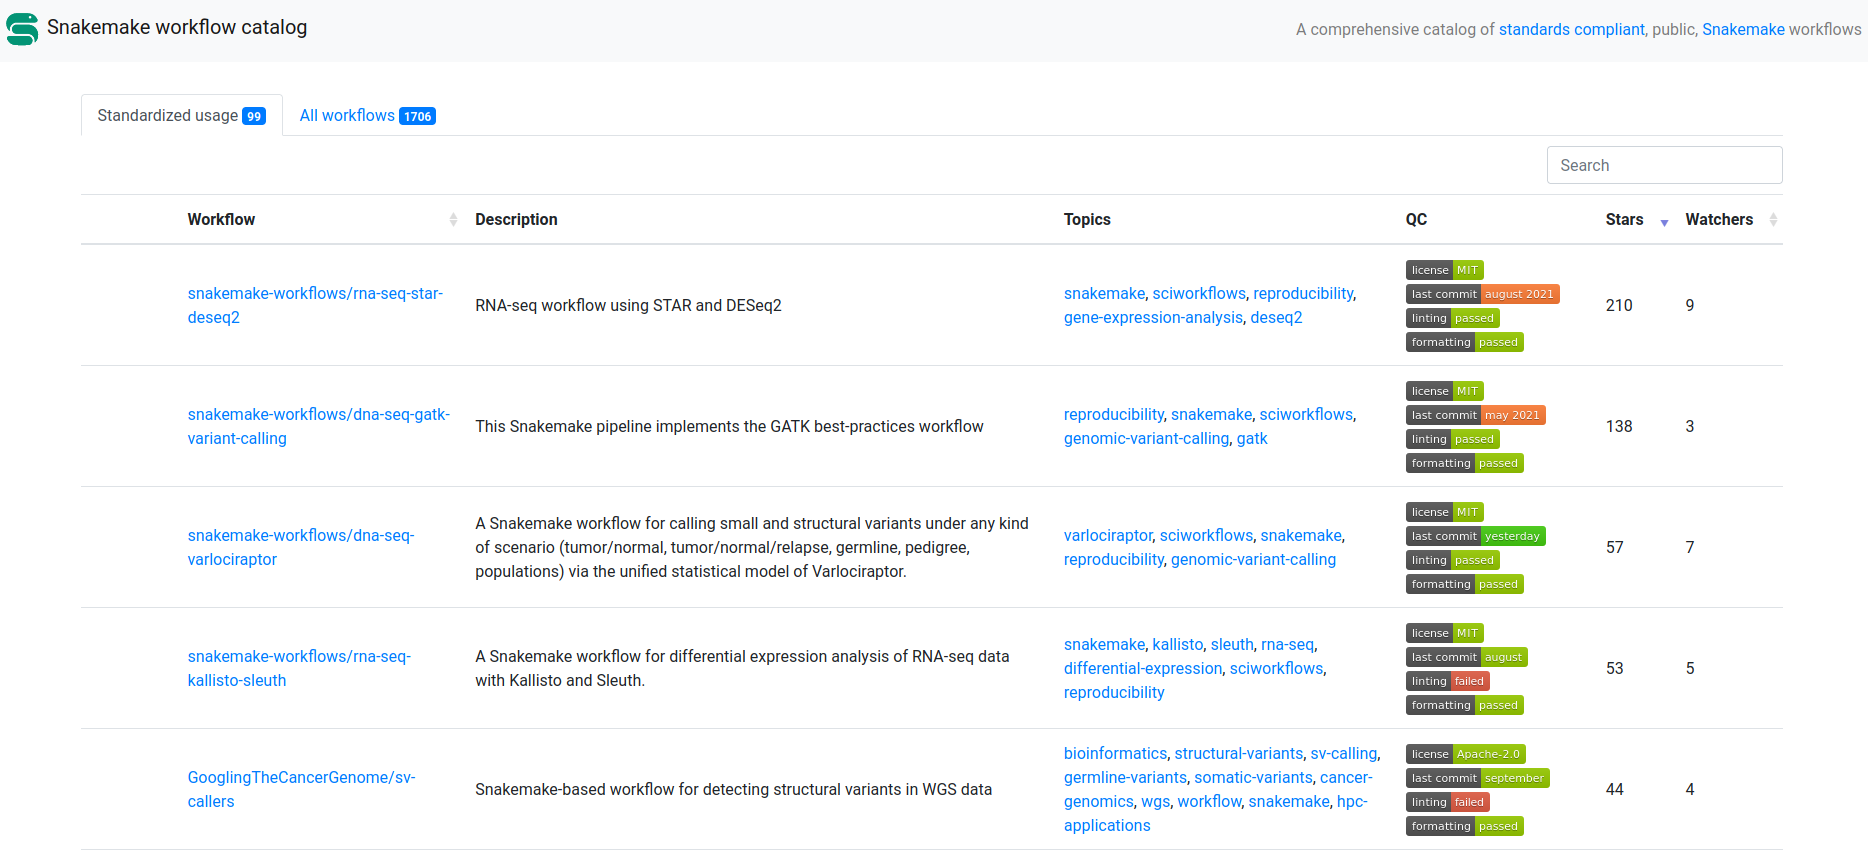
\includegraphics[width=\textwidth]{Snakemake/Snakemake_Workflow_Catalog.png}
        \caption{Screenshot of the Workflow Catalogue}
      \end{figure}
    \end{column}
  \end{columns}
\end{frame}

%%%%%%%%%%%%%%%%%%%%%%%%%%%%%%%%%%%%%%%%%%%%%%%%%%%%%%%%%%%%%%%%%%%%%%%%%%%%%%%%
\begin{frame}[fragile]
  \frametitle{The Tasksetting I}
  We give ourselves a little (proxy) task. Suppose you want to analyse the frequency of words in certain books.\newline
  \pause
  We’ve compiled our raw data i.e. the books we want to analyse and have prepared several Python scripts that together make up our analysis workflow. -- Our example directory is:
  \begin{lstlisting}[language=Bash, style=Shell]
/lustre/project/hpckurs/workflow_course/example/
  \end{lstlisting}
  For starters we just copy the entire directory:
  \begin{lstlisting}[language=Bash, style=Shell]
# create a destination and cd into it
mkdir workflow_course && cd workflow_course
# copy the example directory
$ cp -r /lustre/project/hpckurs/workflow_course/example @.@
  \end{lstlisting}
  \hint{Use TAB-completion to get the entire path typed. Save yourself the mental effort to type!}
\end{frame}

%%%%%%%%%%%%%%%%%%%%%%%%%%%%%%%%%%%%%%%%%%%%%%%%%%%%%%%%%%%%%%%%%%%%%%%%%%%%%%%%
\begin{frame}[fragile]
  \frametitle{The Tasksetting II}
  Now, let us look, what we have here!\newline
  Using the command \texttt{head}, we can have a look in our data, e.\,g.:
  \begin{lstlisting}[language=Bash, style=Shell, basicstyle=\ttfamily\footnotesize]
$ head example/books/isles.txt
  \end{lstlisting}
  To do so, we can cycle throught the history (with the \textuparrow and \textdownarrow keys) and \texttt{[STRG]+a} (or \texttt{[CMD]+a} o an English keyboard to jump to the start of the line and replace \texttt{ls} by \texttt{head}.
  \docs{The \texttt{\textbackslash} is just to allow wrapping the line in \texttt{bash}.}
\end{frame}

%%%%%%%%%%%%%%%%%%%%%%%%%%%%%%%%%%%%%%%%%%%%%%%%%%%%%%%%%%%%%%%%%%%%%%%%%%%%%%%%
\begin{frame}[fragile]
  \frametitle{The Tasksetting III}
  This will (per default) the first 10 lines:
  \begin{lstlisting}[style=Plain, basicstyle=\ttfamily\tiny]
A JOURNEY TO THE WESTERN ISLANDS OF SCOTLAND


INCH KEITH


I had desired to visit the Hebrides, or Western Islands of Scotland, so
long, that I scarcely remember how the wish was originally excited; and
was in the Autumn of the year 1773 induced to undertake the journey, by
finding in Mr. Boswell a companion, whose acuteness would help my
  \end{lstlisting}
  \pause
  \task{Perform the \texttt{head}-command on any other book.}
\end{frame}

%%%%%%%%%%%%%%%%%%%%%%%%%%%%%%%%%%%%%%%%%%%%%%%%%%%%%%%%%%%%%%%%%%%%%%%%%%%%%%%%
\begin{frame}[fragile]
  \frametitle{The Tasksetting IV}
  What else is there?\newline
  We can use the \texttt{tree} command to display the content of an entire directory tree, e.\,g.:
  \begin{lstlisting}[language=Bash, style=Shell]
$ tree example/
  \end{lstlisting}
  \begin{columns}
    \begin{column}{0.2\textwidth}
     Should display
    \end{column}
    \begin{column}{0.8\textwidth}
    \begin{minipage}[t]{0.5\textwidth}
    \setstretch{0.1}
            {\tiny \DTsetlength{0.2em}{1em}{0.2em}{0.4pt}{.6pt}
\dirtree{%
.1 /.
.2 example.
.3 data.
.4 {abyss.txt}\DTcomment{a book}.
.4 {isles.txt}.
.4 {last.txt}.
.4 {sierra.txt}.
.3 scripts.
.4 {plotcount.py}\DTcomment{a script}.
.4 {wordcount.py}.
.4 {zipf\_test.py}.
}}
    \end{minipage}






    \end{column}
  \end{columns}
\end{frame}

%%%%%%%%%%%%%%%%%%%%%%%%%%%%%%%%%%%%%%%%%%%%%%%%%%%%%%%%%%%%%%%%%%%%%%%%%%%%%%%%
\begin{frame}[fragile]
  \frametitle{\Interlude{About Module Files}}
  On HPC Systems Software is provisioned as so-called module files. For example:
  \begin{lstlisting}[language=Bash, style=Shell]
$ module load lang/Python
  \end{lstlisting}
  will load the most recent Python module and provide you with the correct environment.
  \task{Run \texttt{python3 --version}, then load the module and run \texttt{python3 --version} once more.}
>>>>>>> 3344f5544dfc16cd6f382d6d1047efe9fc54b80c
\end{frame}

%%%%%%%%%%%%%%%%%%%%%%%%%%%%%%%%%%%%%%%%%%%%%%%%%%%%%%%%%%%%%%%%%%%%%%%%%%%%%%%%
\begin{frame}[fragile]
  \frametitle{\Interlude{About Module Files II}}
  Eventually we will need a plotting module and a numeric library, too. Please run:
  \begin{lstlisting}[language=Bash, style=Shell]
$ module purge # to get a clean environment again
$ module load vis/matplotlib
  \end{lstlisting}
  \pause
  \question{Which is your version of Python, now?}
\end{frame}

%%%%%%%%%%%%%%%%%%%%%%%%%%%%%%%%%%%%%%%%%%%%%%%%%%%%%%%%%%%%%%%%%%%%%%%%%%%%%%%%
\begin{frame}[fragile]
  \frametitle{The Tasksetting V}
  The first step is to count the words.\newline
  \begin{enumerate}
   \item run \begin{lstlisting}[language=Bash, style=Shell, basicstyle=\footnotesize] 
$ python scripts/wordcount.py -i books/isles.txt -o isles.dat           
             \end{lstlisting}
  \item take a quick look at the results:
        \begin{lstlisting}[language=Bash, style=Shell] 
head -5 isles.dat
        \end{lstlisting}
  \item this shows us the 5 top lines of the result file:
  \begin{lstlisting}[style=Plain]
the 3822 6.7371760973
of 2460 4.33632998414
and 1723 3.03719372466
to 1479 2.60708619778
a 1308 2.30565838181
  \end{lstlisting}
   \end{enumerate}
\end{frame}

%%%%%%%%%%%%%%%%%%%%%%%%%%%%%%%%%%%%%%%%%%%%%%%%%%%%%%%%%%%%%%%%%%%%%%%%%%%%%%%%
\begin{frame}[fragile]
  \frametitle{The Tasksetting VI}
  Let’s visualise the results. The script \texttt{plotcount.py} reads in a data file and plots the 10 most frequently occurring words as a text-based bar plot:
  \begin{lstlisting}[language=Bash, style=Shell] 
$ python scripts/plotcount.py -i isles.dat --type ascii
  \end{lstlisting}
  \pause
  Or your can create a graphical plot:
  \begin{lstlisting}[language=Bash, style=Shell] 
$ python scripts/plotcount.py -i isles.dat -o isles.png
# subsequently run
$ display isles.png
  \end{lstlisting}
  \pause
  Not nice, but it will do ...
\end{frame}

%%%%%%%%%%%%%%%%%%%%%%%%%%%%%%%%%%%%%%%%%%%%%%%%%%%%%%%%%%%%%%%%%%%%%%%%%%%%%%%%
\begin{frame}
  \frametitle{\Interlude{Zipf’s Law}}
  
Zipf’s Law is an empirical law formulated using mathematical statistics that refers to the fact that many types of data studied in the physical and social sciences can be approximated with a Zipfian distribution, one of a family of related discrete power law probability distributions.

Zipf’s law was originally formulated in terms of quantitative linguistics, stating that given some corpus of natural language utterances, the frequency of any word is inversely proportional to its rank in the frequency table. For example, in the Brown Corpus of American English text, the word the is the most frequently occurring word, and by itself accounts for nearly 7\% of all word occurrences (69,971 out of slightly over 1 million). True to Zipf’s Law, the second-place word of accounts for slightly over 3.5\% of words (36,411 occurrences), followed by and (28,852). Only 135 vocabulary items are needed to account for half the Corpus.

Source: \lhref{https://en.wikipedia.org/wiki/Zipf\%27s\_law}{Wikipedia}
\end{frame}

%%%%%%%%%%%%%%%%%%%%%%%%%%%%%%%%%%%%%%%%%%%%%%%%%%%%%%%%%%%%%%%%%%%%%%%%%%%%%%%%
\begin{frame}[fragile]
  \frametitle{The Tasksetting VII}
  Now, we can run our statistical analyis:
  \begin{lstlisting}[language=Bash, style=Shell]
$ python scripts/zipf_test.py isles.dat
  \end{lstlisting}
  \pause
  This means, we can put it all in a \emph{Pipeline} and do our analysis!11!!
  \begin{lstlisting}[language=Bash, style=Shell, basicstyle=\small]
#!/bin/bash
python scripts/wordcount.py -i books/isles.txt -o isles.dat
python scripts/wordcount.py -i books/abyss.txt -o abyss.dat

python scripts/plotcount.py -i isles.dat -o isles.png
python scripts/plotcount.py -i abyss.dat -o abyss.png

# Generate summary table
python scripts/zipf_test.py abyss.dat isles.dat @>@ results.txt
  \end{lstlisting}
  \hint{The \texttt{>} sign is a redirection in \texttt{bash}.}
\end{frame}

%%%%%%%%%%%%%%%%%%%%%%%%%%%%%%%%%%%%%%%%%%%%%%%%%%%%%%%%%%%%%%%%%%%%%%%%%%%%%%%%
\begin{frame}
  \frametitle{Summary}
  This  shell script solves several problems in computational reproducibility:
  \begin{enumerate}[<+->]
   \item It explicitly documents our pipeline, making communication with colleagues (and our future selves) more efficient.
   \item It allows us to type a single command, bash \texttt{run\_pipeline.sh}, to reproduce the full analysis.
   \item It prevents us from repeating typos or mistakes. You might not get it right the first time, but once you fix something it’ll stay fixed.
  \end{enumerate}
  \pause
  \question{What are the shortcomings of this solution?}
\end{frame}

%%%%%%%%%%%%%%%%%%%%%%%%%%%%%%%%%%%%%%%%%%%%%%%%%%%%%%%%%%%%%%%%%%%%%%%%%%%%%%%%
\begin{frame}[fragile]
  \frametitle{Conclusion}
  \begin{enumerate}[<+->]
   \item Suppose you want to change settins of the plot(s). And the compute work would take longer. A manual outcomment would be required.
   \item More inputs will require to add more line or be clever with loops, e.\,g.:
         \begin{lstlisting}[language=Bash, style=Shell]
for book in books/*txt; do 
  python scripts/wordcount.py -i ${book} -o {book/txt/png}
done
         \end{lstlisting}
  \end{enumerate}
  Or something similar ...\newline
  What we \emph{really} want is an executable description of our pipeline that allows software to do the tricky part for us: figuring out what tasks need to be run where and when, then perform those tasks for us.
\end{frame}

%%%%%%%%%%%%%%%%%%%%%%%%%%%%%%%%%%%%%%%%%%%%%%%%%%%%%%%%%%%%%%%%%%%%%%%%%%%%%%%%
\begin{frame}[fragile]
  \frametitle{One last Thing}
  Please delete all previous outputs:
  \begin{lstlisting}[language=Bash, style=Shell]
rm *dat *png 
  \end{lstlisting}
  \hint{\texttt{Snakemake} will recognize existing outputs and skip processes, which would be redundant.}
\end{frame}






%%%%%%%%%%%%%%%%%%%%%%%%%%%%%%%%%%%%%%%%%%%%%%%%%%%%%%%%%%%%%%%%%%%%%%%%%%%%%%%%
%%%%%%%%%%%%%%%%%%%%%%%%%%%%%%%%%%%%%%%%%%%%%%%%%%%%%%%%%%%%%%%%%%%%%%%%%%%%%%%%
\section{A first Workflow}

%%%%%%%%%%%%%%%%%%%%%%%%%%%%%%%%%%%%%%%%%%%%%%%%%%%%%%%%%%%%%%%%%%%%%%%%%%%%%%%%
\begin{frame}
    \frametitle{Outline}
    \begin{columns}[t]
        \begin{column}{.5\textwidth}
            \tableofcontents[sections={1-7},currentsection]
        \end{column}
        \begin{column}{.5\textwidth}
            \tableofcontents[sections={8-15},currentsection]
        \end{column}
    \end{columns}
\end{frame}

%%%%%%%%%%%%%%%%%%%%%%%%%%%%%%%%%%%%%%%%%%%%%%%%%%%%%%%%%%%%%%%%%%%%%%%%%%%%%%%%
\begin{frame}
  \frametitle{What is this about?}
   \begin{question}[Questions]
   	 How do I write a simple workflow?
   \end{question}
   \begin{docs}[Objectives]
   	 \begin{enumerate}
                      \item Understand the components of a Snakefile: rules, inputs, outputs, and actions.
                      \item Write a simple Snakefile.
                      \item Run Snakemake from the shell.
     \end{enumerate}
   \end{docs}
\end{frame}

%%%%%%%%%%%%%%%%%%%%%%%%%%%%%%%%%%%%%%%%%%%%%%%%%%%%%%%%%%%%%%%%%%%%%%%%%%%%%%%
\begin{frame}[fragile]
  \frametitle{Before we begin \ldots}
  \begin{exampleblock}{Working with closure Files}
    To ease the excercises and save typing time, all exercises are supplied as cloze texts.\linebreak
    \Snakemake{} relies on a file called \Snakemake{} to be present. You can either rename your cloze texts like
    \begin{lstlisting}[language=Bash, style=Shell]
$ cp <number>_Snakefile Snakefile
    \end{lstlisting}
    or specify the workflow file on the command line with an additional flag:
    \begin{lstlisting}[language=Bash, style=Shell]
$ snakemake <other arguments> \
> --snakefile <number>_Snakefile
    \end{lstlisting}
    Also note: \altverb{\\} may denote a linebreak in \texttt{Bash} and \altverb{>} its continuation. Omit these and you have a one-liner. It merely serves to fit text on screen, here.
  \end{exampleblock}
\end{frame}


%%%%%%%%%%%%%%%%%%%%%%%%%%%%%%%%%%%%%%%%%%%%%%%%%%%%%%%%%%%%%%%%%%%%%%%%%%%%%%%%
\subsection{A first Step or ``Rule''}

%%%%%%%%%%%%%%%%%%%%%%%%%%%%%%%%%%%%%%%%%%%%%%%%%%%%%%%%%%%%%%%%%%%%%%%%%%%%%%%%
\begin{frame}[fragile]
  \frametitle{Layout of a Workflow Development Directory} 
  The idea is to have a neat overview:
  \begin{columns}
    \begin{column}{0.5\textwidth}
      
  \begin{minipage}[t]{0.5\textwidth}
    \setstretch{0.1}
            {\tiny \DTsetlength{0.2em}{1em}{0.2em}{0.4pt}{.6pt}
\dirtree{%
.1 {\textit{workflow\ folder}}.
.2 {scripts}.
.3 {some\ scriptfile.py}.
.3 {some\ scriptfile.sh}.
.3 {some\ scriptfile.R}.
.2 {Snakefile}.
.2 {and more \ldots}.
}}
    \end{minipage}
    \end{column}
    \begin{column}{0.5\textwidth}
      \begin{hint}
      	Our long term goal:\newline Have a orderly overview and seperation of data and code. We will start with one \altverb{Snakefile}.
      \end{hint}
    \end{column}
  \end{columns}
\end{frame}

%%%%%%%%%%%%%%%%%%%%%%%%%%%%%%%%%%%%%%%%%%%%%%%%%%%%%%%%%%%%%%%%%%%%%%%%%%%%%%%%
\begin{frame}[fragile]
  \frametitle{Our first \altverb{Snakefile}!}
  \begin{onlyenv}<1| handout:0>
    Our first ``\altverb{rule}''; we want to map reads onto a reference genome. 
    \begin{lstlisting}[language=Python,style=Python]
rule bwa_map:
    input:
        "data/genome.fa",
        "data/samples/A.fastq"
    output:
        "mapped_reads/A.bam"
    shell:
        "bwa mem data/genome.fa"
        " data/samples/A.fastq"
        " | samtools view -Sb - >"
        " mapped_reads/A.bam"
    \end{lstlisting}
    \begin{docs}
    	This code is build file, which for \Snakemake{} is called a \altverb{Snakefile} -- a file executed by \Snakemake{}.
    \end{docs}
    \end{onlyenv}
  \begin{onlyenv}<2| handout:0>
   We are going to ``map'' our reads onto the genome.
   \begin{lstlisting}[language=Python,style=Python]
rule @bwa_map@:
    input:
        "data/genome.fa",
        "data/samples/A.fastq"
    output:
        "mapped_reads/A.bam"
    shell:
        "bwa mem data/genome.fa"
        " data/samples/A.fastq"
        " | samtools view -Sb - >"
        " mapped_reads/A.bam"
    \end{lstlisting}
    For this we are using \lhref{https://github.com/lh3/bwa}{\altverb{bwa}}, specifically \altverb{bwa mem}. We call our rule accordingly \altverb{bwa_map}.
  \end{onlyenv}
  \begin{onlyenv}<3| handout:0>
   \altverb{input}, \altverb{output} and \altverb{shell} are called ``directives'':
   \begin{lstlisting}[language=Python,style=Python]
rule bwa_map:
    @input@:
        "data/genome.fa",
        "data/samples/A.fastq"
    @output@:
        "mapped_reads/A.bam"
    @shell@:
        "bwa mem data/genome.fa"
        " data/samples/A.fastq"
        " | samtools view -Sb - >"
        " mapped_reads/A.bam"
    \end{lstlisting}
    The \altverb{input} and \altverb{output} directives are followed by lists of files that are expected to be used or created by the rule. In the simplest case, these are just explicit Python strings.
  \end{onlyenv}
  \begin{onlyenv}<4| handout:0>
   The \altverb{shell} may be one line or contain line breaks:
  \begin{lstlisting}[language=Python,style=Python]
rule bwa_map:
    input:
        "data/genome.fa",
        "data/samples/A.fastq"
    output:
        "mapped_reads/A.bam"
    shell:
        @"bwa mem data/genome.fa"
        " data/samples/A.fastq"
        " | samtools view -Sb - >"
        " mapped_reads/A.bam"@
    \end{lstlisting}
    \bcattention Python will concatenate those Strings! Be sure to include spaces to make up a valid command in Bash.
  \end{onlyenv}
  \begin{onlyenv}<5| handout:1>
   Be sure to have copied everything to your \altverb{Snakefile} and save it.
   \begin{lstlisting}[language=Python,style=Python]
rule bwa_map:
    input:
        "data/genome.fa",
        "data/samples/A.fastq"
    output:
        "mapped_reads/A.bam"
    shell:
        "bwa mem data/genome.fa"
        " data/samples/A.fastq"
        " | samtools view -Sb - >"
        " mapped_reads/A.bam"
    \end{lstlisting}
    You will find the working content in \altverb{01_Snakefile}, too.
  \end{onlyenv}
\end{frame}

%%%%%%%%%%%%%%%%%%%%%%%%%%%%%%%%%%%%%%%%%%%%%%%%%%%%%%%%%%%%%%%%%%%%%%%%%%%%%%%%
\begin{frame}
  \frametitle{\altverb{Snakefile}s are Python Files}
  \begin{block}{Some Background}
     \begin{enumerate}
       \item Like Python, you can use either tabs or spaces for indentation — don’t mix! Consensus is to only use spaces.
       \item Together, the target, dependencies, and actions form a rule. A rule is a recipe for how to make things.
  \end{enumerate}
  \end{block}
\end{frame}

%%%%%%%%%%%%%%%%%%%%%%%%%%%%%%%%%%%%%%%%%%%%%%%%%%%%%%%%%%%%%%%%%%%%%%%%%%%%%%%%
\begin{frame}[fragile]
  \frametitle{Testing our \altverb{Snakefile}}
  When a workflow is executed, \Snakemake{} tries to generate given target files. Target files can be specified via the command line. By executing
  \begin{lstlisting}[language=Bash, style=Shell]
$ snakemake -np mapped_reads/A.bam
  \end{lstlisting}
  in the working directory containing the \altverb{Snakefile}, we tell \Snakemake{} to generate the target file \altverb{mapped_reads/A.bam}.\newline
  We are using 
  \begin{itemize}[<+->]
   \item \altverb{-n/--dry-run} to show the \emph{planned} execution and
   \item \altverb{-p} to print the intended shell command.
  \end{itemize} 
\end{frame}

%%%%%%%%%%%%%%%%%%%%%%%%%%%%%%%%%%%%%%%%%%%%%%%%%%%%%%%%%%%%%%%%%%%%%%%%%%%%%%%%
\begin{frame}[fragile]
  \frametitle{Finally - Running \Snakemake{}!}
  Now, we can run \Snakemake{}:
  \begin{lstlisting}[language=Bash, style=Shell]
$ snakemake --cores=1 mapped_reads/A.bam
  \end{lstlisting}
  \begin{hint}[Note:]
  	The \altverb{--cores=1} is necessary, because we are executing ``locally'' and \Snakemake{} would like to know how much of the resources we may use (you can try without, though, to see what happens).
  \end{hint}
  You should see the expected output (\altverb[Bash]{ls}) and lines which reads:
  \begin{lstlisting}[style=Plain, basicstyle=\footnotesize]
1 of 1 steps (100%) done
Complete log: .snakemake/log/2022-09-17T145657.968906.snakemake.log
  \end{lstlisting}
\end{frame}

%%%%%%%%%%%%%%%%%%%%%%%%%%%%%%%%%%%%%%%%%%%%%%%%%%%%%%%%%%%%%%%%%%%%%%%%%%%%%%%%
\begin{frame}[fragile]
  \frametitle{Re-Running Workflows}
  Try to run \Snakemake{} again:
  \begin{lstlisting}[language=Bash, style=Shell]
$ snakemake --cores=1 mapped_reads/A.bam
  \end{lstlisting}
  \pause
  Oops:
  \begin{lstlisting}[style=Plain, basicstyle=\footnotesize]
Nothing to be done (all requested files are present and up to date).
  \end{lstlisting}
  \pause
  Now, do:
  \begin{lstlisting}[language=Bash, style=Shell]
$ touch mapped_reads/A.bam
  \end{lstlisting}
  And run \Snakemake{} once more.
  \begin{question}
  	What happens? Why?
  \end{question}
\end{frame}

%%%%%%%%%%%%%%%%%%%%%%%%%%%%%%%%%%%%%%%%%%%%%%%%%%%%%%%%%%%%%%%%%%%%%%%%%%%%%%%%
\begin{frame}
  \frametitle{When do Rules get executed? - The Solution}
  When it is asked to build a target, \Snakemake{} checks the “last modification time” of both the \emph{target} and its \emph{dependencies}.
  If either
  \begin{itemize}
   \item any dependency has been updated
   \item or a job failed to produce a target (completely)
  \end{itemize}
  upon re-run \Snakemake{} will only rebuild the files that, either directly or indirectly, depend on the file that changed. This is called an \emph{incremental build}.
  \pause
  \begin{docs}
  	By explicitly recording the inputs to and outputs from steps in our analysis and the dependencies between files, \altverb{Snakefile}s act as a type of documentation, reducing the number of things we have to remember.
  \end{docs}
\end{frame}

%%%%%%%%%%%%%%%%%%%%%%%%%%%%%%%%%%%%%%%%%%%%%%%%%%%%%%%%%%%%%%%%%%%%%%%%%%%%%%%%
\begin{frame}[fragile]
  \frametitle{Too much Typing!1!11!}
  A closer look on our first rule reveals:
  \begin{lstlisting}[language=Python,style=Python]
rule bwa_map:
    input:
        "data/genome.fa",
        "data/samples/A.fastq"
    output:
        "mapped_reads/A.bam"
    shell:
        "bwa mem data/genome.fa"
        " data/samples/A.fastq"
        " | samtools view -Sb - >"
        " mapped_reads/A.bam"
    \end{lstlisting}
    \bcattention Way too much redundancy!
\end{frame}

%%%%%%%%%%%%%%%%%%%%%%%%%%%%%%%%%%%%%%%%%%%%%%%%%%%%%%%%%%%%%%%%%%%%%%%%%%%%%%%%
\begin{frame}[fragile]
  \frametitle{Introducing Wildcards}
  \altverb{input} and \altverb{output} can be referenced in our file, with an expression called ``wildcard'':
  \begin{lstlisting}[language=Python,style=Python]
rule bwa_map:
    input:
        "data/genome.fa",
        "data/samples/A.fastq"
    output:
        "mapped_reads/A.bam"
    shell:
        "bwa mem {input}"
        " | samtools view -Sb - >"
        " {output}"
    \end{lstlisting}
    Since the rule has multiple input files, \Snakemake{} will concatenate them, separated by a whitespace. In other words, \Snakemake{} will replace \altverb{\{input\}} with \altverb{data/genome.fa data/samples/A.fastq} before executing the command.\newline
    A working example can be found in \altverb{02_Snakefile}.
\end{frame}

%%%%%%%%%%%%%%%%%%%%%%%%%%%%%%%%%%%%%%%%%%%%%%%%%%%%%%%%%%%%%%%%%%%%%%%%%%%%%%%%
\begin{frame}[fragile]
  \frametitle{Further Workflow Decoration}\footnotesize 
  \Snakemake{} allows generalizing rules by using named wildcards. Simply replace the \altverb{A} in the second input file and in the output file with the wildcard \altverb{\{sample\}}, to yield:
  \begin{lstlisting}[language=Python,style=Python,basicstyle=\footnotesize]
rule bwa_map:
    input:
        "data/genome.fa",
        "data/samples/{sample}.fastq"
    output:
        "mapped_reads/{sample}.bam"
    shell:
        "bwa mem {input} | samtools view -Sb - > {output}"
  \end{lstlisting}
  When \Snakemake{} determines that this rule can be applied to generate a target file by replacing the wildcard \altverb{\{sample\}} in the output file with an appropriate value, it will propagate that value to all occurrences of \altverb{\{sample\}} in the input files and thereby determine the necessary input for the resulting job. 
\end{frame}

%%%%%%%%%%%%%%%%%%%%%%%%%%%%%%%%%%%%%%%%%%%%%%%%%%%%%%%%%%%%%%%%%%%%%%%%%%%%%%%%
\begin{frame}
  \frametitle{One Caveat!}
  \begin{alertblock}{Multiple Wildcards}
    You can have multiple wildcards in your file paths, however, to avoid conflicts with other jobs of the same rule, \emph{all output files} of a rule \emph{have to contain exactly the same wildcards}.
  \end{alertblock}
\end{frame}

%%%%%%%%%%%%%%%%%%%%%%%%%%%%%%%%%%%%%%%%%%%%%%%%%%%%%%%%%%%%%%%%%%%%%%%%%%%%%%%%
\begin{frame}[fragile]
  \frametitle{Execution}
  When executing
  \begin{lstlisting}[language=Bash, style=Shell]
$ snakemake -np mapped_reads/B.bam
  \end{lstlisting}
  \Snakemake{} will determine that the rule \altverb{bwa_map} can be applied to generate the target file by replacing the wildcard \altverb{\{sample\}} with the value \altverb{B}.\newline
  To analyse samples \altverb{A} and \altverb{B}, we can specify two targets
    \begin{lstlisting}[language=Bash, style=Shell]
$ snakemake -np mapped_reads/A.bam mapped_reads/B.bam
  \end{lstlisting}
  or use \lhref{https://tldp.org/LDP/Bash-Beginners-Guide/html/sect_03_04.html}{Bash's brace expansion}
  \begin{lstlisting}[language=Bash, style=Shell]
$ snakemake -np mapped_reads/{A,B}.bam
  \end{lstlisting}
\end{frame}

%%%%%%%%%%%%%%%%%%%%%%%%%%%%%%%%%%%%%%%%%%%%%%%%%%%%%%%%%%%%%%%%%%%%%%%%%%%%%%%%
\begin{frame}[fragile]
  \frametitle{Sorting Alignments}
  For later steps, we need the read alignments in the BAM files to be sorted. This can be achieved with the \lhref{https://www.htslib.org/}{\texttt{samtools}} \altverb{sort} command. We add the following rule beneath the \altverb{bwa_map} rule:
  \begin{lstlisting}[language=Python,style=Python]
rule samtools_sort:
    input:
        "mapped_reads/{sample}.bam"
    output:
        "sorted_reads/{sample}.bam"
    shell:
        "samtools sort -T sorted_reads/{wildcards.sample} "
        "-O bam {input} > {output}"
  \end{lstlisting}
  %TODO check cloze text correct?
  \begin{task}
  	Please refer to your template \altverb{03_Snakefile}.
  \end{task}
\end{frame}

%%%%%%%%%%%%%%%%%%%%%%%%%%%%%%%%%%%%%%%%%%%%%%%%%%%%%%%%%%%%%%%%%%%%%%%%%%%%%%%%
\begin{frame}[fragile]
  \frametitle{Using Wildcards}
  The rule will take  input file from the \altverb{mapped_reads} directory and store a sorted version in the \altverb{sorted_reads} directory.
  \pause
  \begin{docs}
  	\Snakemake{} will automatically create missing directories!
  \end{docs}
  You noticed \altverb{-T sorted_reads/\{wildcards.sample\}}?
  \pause
  For sorting, \texttt{samtools} requires a prefix specified with the flag \altverb{-T}. Here, we need the value of the wildcard \altverb{sample}. \Snakemake{} allows to access wildcards in the shell command via the wildcards object that has an attribute with the value for each wildcard.
\end{frame}

%%%%%%%%%%%%%%%%%%%%%%%%%%%%%%%%%%%%%%%%%%%%%%%%%%%%%%%%%%%%%%%%%%%%%%%%%%%%%%%%
\begin{frame}[fragile]
  \frametitle{Execution}
  When you run 
  \begin{lstlisting}[language=Bash, style=Shell]
$ snakemake -np sorted_reads/B.bam
  \end{lstlisting}
  you will notice that \Snakemake{} wants to run the first rule \altverb{bwa_map} and then the rule \altverb{samtools_sort} to create the desired target file.
  \begin{docs}
  	Dependencies are resolved automatically by matching file names.
  \end{docs}
\end{frame}

%%%%%%%%%%%%%%%%%%%%%%%%%%%%%%%%%%%%%%%%%%%%%%%%%%%%%%%%%%%%%%%%%%%%%%%%%%%%%%%%
\begin{frame}[fragile]
  \frametitle{Indexing Read Alignments}
  We need to use samtools again to index the sorted read alignments so that we can quickly access reads by the genomic location they were mapped to. This can be done with the following rule:
  \begin{lstlisting}[language=Python,style=Python]
rule samtools_index:
    input:
        "sorted_reads/{sample}.bam"
    output:
        "sorted_reads/{sample}.bam.bai"
    shell:
        "samtools index {input}"
  \end{lstlisting}
  \begin{hint}[Note]
  	You will find this code in the next cloze text. It is not worth proceeding without the next step.
  \end{hint}
\end{frame}

%%%%%%%%%%%%%%%%%%%%%%%%%%%%%%%%%%%%%%%%%%%%%%%%%%%%%%%%%%%%%%%%%%%%%%%%%%%%%%%%
\begin{frame}[fragile]
 \frametitle{Calling Genomic Variants - Background I}
 The next step in our workflow will aggregate the mapped reads from all samples and jointly call genomic variants on them. We need two tools: \lhref{https://www.htslib.org/}{samtools} and \lhref{https://www.htslib.org/}{bcftools}. \newline \pause
 \Snakemake{} provides a helper function for collecting input files that helps us to describe the aggregation in this step. With
 \begin{lstlisting}[language=Python,style=Python]
expand("sorted_reads/{sample}.bam", sample=SAMPLES)
 \end{lstlisting}
 we obtain a list where the given pattern \altverb{sorted_reads/\{sample\}.bam} was formatted with the values in a given list of samples \altverb{SAMPLES}, i.\,e.
 \begin{lstlisting}[language=Python,style=Python]
["sorted_reads/A.bam", "sorted_reads/B.bam"]
 \end{lstlisting}
\end{frame}

%%%%%%%%%%%%%%%%%%%%%%%%%%%%%%%%%%%%%%%%%%%%%%%%%%%%%%%%%%%%%%%%%%%%%%%%%%%%%%%%
\begin{frame}[fragile]
 \frametitle{Calling Genomic Variants - Background II}
 This is particularly useful when dealing with \emph{multiple} wildcards, e.\,g.:
 \begin{lstlisting}[language=Python,style=Python]
expand("sorted_reads/{sample}.{replicate}.bam", 
          sample=SAMPLES, replicate=[0, 1])
 \end{lstlisting}
 With all elements of \altverb{SAMPLES} and the list \altverb{[0, 1]}, we get:
 \begin{lstlisting}[language=Python,style=Python]
["sorted_reads/A.0.bam", "sorted_reads/A.1.bam", 
 "sorted_reads/B.0.bam", "sorted_reads/B.1.bam"]
 \end{lstlisting}
\end{frame}
  
%%%%%%%%%%%%%%%%%%%%%%%%%%%%%%%%%%%%%%%%%%%%%%%%%%%%%%%%%%%%%%%%%%%%%%%%%%%%%%%%
\begin{frame}[fragile]
  \frametitle{Calling Genomic Variants}
  Later, we will learn how to provide input more sophistically \ldots\newline
  For now, we will define a list on top of our \altverb{Snakefile}:
  \begin{lstlisting}[language=Python,style=Python]
SAMPLES = ["A", "B"]
  \end{lstlisting}
  Now, we can add the following rule to our \altverb{Snakefile}:
  \begin{lstlisting}[language=Python,style=Python,basicstyle=\footnotesize]
rule bcftools_call:
    input:
        fa="data/genome.fa",
        bam=@expand("sorted_reads/{sample}.bam", sample=SAMPLES),@
        bai=@expand("sorted_reads/{sample}.bam.bai", sample=SAMPLES)@
    output:
        "calls/all.vcf"
    shell:
        "bcftools mpileup -f {input.fa} {input.bam} | "
        "bcftools call -mv - > {output}"
  \end{lstlisting}
  This is part of \altverb{05_Snakefile}.
\end{frame}





%%%%%%%%%%%%%%%%%%%%%%%%%%%%%%%%%%%%%%%%%%%%%%%%%%%%%%%%%%%%%%%%%%%%%%%%%%%%%%%%
%%%%%%%%%%%%%%%%%%%%%%%%%%%%%%%%%%%%%%%%%%%%%%%%%%%%%%%%%%%%%%%%%%%%%%%%%%%%%%%%
\section{Wildcards for more elegant Workflows}

%%%%%%%%%%%%%%%%%%%%%%%%%%%%%%%%%%%%%%%%%%%%%%%%%%%%%%%%%%%%%%%%%%%%%%%%%%%%%%%%
\begin{frame}
    \frametitle{Outline}
    \begin{columns}[t]
        \begin{column}{.5\textwidth}
            \tableofcontents[sections={1-9},currentsection]
        \end{column}
        \begin{column}{.5\textwidth}
            \tableofcontents[sections={10-18},currentsection]
        \end{column}
    \end{columns}
\end{frame}

%%%%%%%%%%%%%%%%%%%%%%%%%%%%%%%%%%%%%%%%%%%%%%%%%%%%%%%%%%%%%%%%%%%%%%%%%%%%%%%%
\begin{frame}
  \frametitle{What is this about?}
   \question[Questions]{\begin{itemize}
                         \item The workflow still is pretty verbose, how can we be more concise?
                         \item How can the redundancy in a workflow be reduced?
                        \end{itemize}
                       }
   \docs[Objectives]{\begin{enumerate}
                      \item Use \texttt{Snakemake} wildcards to simplify our rules.
                      \item Output files are a product not only of input files but of the scripts or code that created the output files.
                     \end{enumerate}}
\end{frame}

%%%%%%%%%%%%%%%%%%%%%%%%%%%%%%%%%%%%%%%%%%%%%%%%%%%%%%%%%%%%%%%%%%%%%%%%%%%%%%%%
\subsection{Better In-/Output}

%%%%%%%%%%%%%%%%%%%%%%%%%%%%%%%%%%%%%%%%%%%%%%%%%%%%%%%%%%%%%%%%%%%%%%%%%%%%%%%%
\begin{frame}
  \frametitle{Rule number One: Don't repeat Yourself!}

Our \texttt{Snakefile} has enormous redundancy: 
\begin{itemize}
 \item names of in-/output files are repeated
 \item rules for every in-/output
\end{itemize}
\docs{\texttt{Snakefile}s are a form of code and, in any code, repeated code can lead to problems (e.g. we rename a data file in one part of the \texttt{Snakefile} but forget to rename it elsewhere).}
\end{frame}

%%%%%%%%%%%%%%%%%%%%%%%%%%%%%%%%%%%%%%%%%%%%%%%%%%%%%%%%%%%%%%%%%%%%%%%%%%%%%%%%
\subsection{Wildcards}

%%%%%%%%%%%%%%%%%%%%%%%%%%%%%%%%%%%%%%%%%%%%%%%%%%%%%%%%%%%%%%%%%%%%%%%%%%%%%%%%
\begin{frame}[fragile]
  \frametitle{The \texttt{\{output\}} Wildcard}
  Consider our last rule
  \begin{lstlisting}[language=Python,style=Python]
# generate summary table
rule zipf_test:
    input:  'abyss.dat', 'last.dat', 'isles.dat'
    output: 'results.txt'
    shell:  'python scripts/zipf_test.py' 
            ' abyss.dat isles.dat last.dat > results.txt'
  \end{lstlisting}
  We can replace the result name first with the wildcard \altverb{\{output\}}:
  \begin{lstlisting}[language=Python,style=Python]
# generate summary table
rule zipf_test:
    input:  'abyss.dat', 'last.dat', 'isles.dat'
    output: 'results.txt'
    shell:  'python scripts/zipf_test.py' 
            ' abyss.dat isles.dat last.dat > {output}'
  \end{lstlisting}
\end{frame}

%%%%%%%%%%%%%%%%%%%%%%%%%%%%%%%%%%%%%%%%%%%%%%%%%%%%%%%%%%%%%%%%%%%%%%%%%%%%%%%%
\begin{frame}[fragile]
  \frametitle{The \texttt{\{input\}} Wildcard}
  Likewise, we may choose to replace our inputs:
  \begin{lstlisting}[language=Python,style=Python]
# generate summary table
rule zipf_test:
    input:  'abyss.dat', 'last.dat', 'isles.dat'
    output: 'results.txt'
    shell:  'python scripts/zipf_test.py' 
            ' {input} > {output}'
  \end{lstlisting}
  Here, \altverb{\{input\}} will contain the entire list of inputs!
\end{frame}

%%%%%%%%%%%%%%%%%%%%%%%%%%%%%%%%%%%%%%%%%%%%%%%%%%%%%%%%%%%%%%%%%%%%%%%%%%%%%%%%
\begin{frame}[fragile]
  \frametitle{The \texttt{\{input\}} Wildcard - II}
  We have learned that
  \begin{lstlisting}[language=Python,style=Python]
rule <rulename>:
  input: <file1>, <file2>, ... <file_n>
  \end{lstlisting}
  translates to a list which we can access as
  \begin{lstlisting}[language=Python,style=Python]
  shell: 'cmd {input}'
  \end{lstlisting}
  As it is a list, we can access individual items by index, too. E.\,g.:
  \begin{lstlisting}[language=Python,style=Python]
  shell: 'cmd --reference {input[0} -i {input[1]}'
  \end{lstlisting}
\end{frame}

%%%%%%%%%%%%%%%%%%%%%%%%%%%%%%%%%%%%%%%%%%%%%%%%%%%%%%%%%%%%%%%%%%%%%%%%%%%%%%%%
\begin{frame}[fragile]
  \frametitle{The  \texttt{\{input\}} Wildcard - III}
  So, \altverb{\{input\}}, can be a single item, a list (accessible by index) or named. For example:
  \begin{lstlisting}[language=Python,style=Python]
rule <rulename>:
  input:
    reference: <path to reference>
    forward:   <path to forward reads>
    reverse:   <path to reverse reads>
  # minimap2 is just an example
  shell: 'minimap2 {reference} {forward}' 
         ' {reverse} > {output}'
  \end{lstlisting}
  \pause
  \altverb{\{output\}} follows the same rules, so for both the options are:
  \begin{itemize}
   \item single item
   \item list (accessible by index)
   \item named access
  \end{itemize}
\end{frame}

%%%%%%%%%%%%%%%%%%%%%%%%%%%%%%%%%%%%%%%%%%%%%%%%%%%%%%%%%%%%%%%%%%%%%%%%%%%%%%%%
\begin{frame}[fragile]
  We \emph{could} write:
  \begin{lstlisting}[language=Python,style=Python]
rule count_words:
    input:
        wc='scripts/wordcount.py',
        book='../books/{file}.txt'
    output: '{file}.dat'
    shell:  'python {input.wc} {input.book} {output}'
  \end{lstlisting}
  \explanation{\altverb{\{file\}} is another arbitrary wildcard, that we can use as a placeholder for any generic book to analyse. Note that we don’t have to use \emph{``file''} as the name of our wildcard — it can be anything we want! Condition: Only available for \altverb{input} and \altverb{output}, not for actions!}
\end{frame}

%%%%%%%%%%%%%%%%%%%%%%%%%%%%%%%%%%%%%%%%%%%%%%%%%%%%%%%%%%%%%%%%%%%%%%%%%%%%%%%%
\begin{frame}[fragile]
  So, we had:
    \begin{lstlisting}[language=Python,style=Python]
  rule count_words:
    input:
        wc='scripts/wordcount.py',
        book='../books/{file}.txt'
    output: '{file}.dat'
    shell:  'python {input.wc} {input.book} {output}'   
    \end{lstlisting}
    \begin{block}{This rule can be interpreted as:}
``In order to build a file named \altverb{something.dat} (the output) find a file named \altverb{../books/something.txt} (the input) and run \altverb{wordcount.py input output}.''
  \end{block}
\end{frame}

%%%%%%%%%%%%%%%%%%%%%%%%%%%%%%%%%%%%%%%%%%%%%%%%%%%%%%%%%%%%%%%%%%%%%%%%%%%%%%%%
\begin{frame}[fragile]
  \frametitle{\HandsOn{Using the \texttt{\{input\}} and \texttt{\{output\}} wildcards!}}
  \begin{enumerate}
   \item Re-write the current workflow to be using the \altverb{\{input\}} and \altverb{\{output\}} wildcards.
   \item Remember: This only needs to be in the \altverb{shell} commands.
   \item Also, use the \altverb{\{file\}} wildcard to reduce the \altverb{count...} rules to just \altverb{count_words} for all inputs.
   \item For this, remember:
         \begin{lstlisting}[language=Python,style=Python]
rule ...:
    input: '../books/{file}.txt'
    output: '{file}.dat'
         \end{lstlisting}
         to be combined with the \altverb{\{input\}} and \altverb{\{output\}} wildcards in the \altverb{shell} part.
  \end{enumerate}
  \hint{Refer to \texttt{04\_Snakefile} as the cloze text.}
\end{frame}


%%%%%%%%%%%%%%%%%%%%%%%%%%%%%%%%%%%%%%%%%%%%%%%%%%%%%%%%%%%%%%%%%%%%%%%%%%%%%%%%
\begin{frame}[fragile]
Our little exercise should produce this Workflow:
      \begin{lstlisting}[language=Python,style=Python, basicstyle=\tiny]
rule dats:
     input:
        'results.txt'

# delete everything so we can re-run things
rule clean:
    shell: 'rm -f *.dat'

rule count_words:
    input:  '../books/{file}.txt'
    output: '{file}.dat'
    shell:  'python scripts/wordcount.py -i {input} -o {output}'
    
# generate summary table
rule zipf_test:
    input: "abyss.dat", "isles.dat", "last.dat"
    output: 'results.txt'
    shell:  
        'scripts/zipf_test.py  {input} > {output}'
      \end{lstlisting}

\end{frame}


%%%%%%%%%%%%%%%%%%%%%%%%%%%%%%%%%%%%%%%%%%%%%%%%%%%%%%%%%%%%%%%%%%%%%%%%%%%%%%%%
%%%%%%%%%%%%%%%%%%%%%%%%%%%%%%%%%%%%%%%%%%%%%%%%%%%%%%%%%%%%%%%%%%%%%%%%%%%%%%%%
\section{Snakefiles as Python-Code}

%%%%%%%%%%%%%%%%%%%%%%%%%%%%%%%%%%%%%%%%%%%%%%%%%%%%%%%%%%%%%%%%%%%%%%%%%%%%%%%%
\begin{frame}
    \frametitle{Outline}
    \begin{columns}[t]
        \begin{column}{.5\textwidth}
            \tableofcontents[sections={1-7},currentsection]
        \end{column}
        \begin{column}{.5\textwidth}
            \tableofcontents[sections={8-15},currentsection]
        \end{column}
    \end{columns}
\end{frame}

%%%%%%%%%%%%%%%%%%%%%%%%%%%%%%%%%%%%%%%%%%%%%%%%%%%%%%%%%%%%%%%%%%%%%%%%%%%%%%%%
\begin{frame}
  \frametitle{What is this about?}
   \begin{question}[Questions]
   	 \begin{itemize}
        \item How can I automatically manage dependencies and outputs?
        \item How can I use Python code to add features to my pipeline?
     \end{itemize}
   \end{question}
   \begin{docs}[Objectives]
   	  \begin{enumerate}
                      \item Use variables, functions, and imports in a Snakefile. 
                      \item Learn to use the \texttt{run} action to execute Python code as an action.
       \end{enumerate}
   \end{docs}
\end{frame}

%%%%%%%%%%%%%%%%%%%%%%%%%%%%%%%%%%%%%%%%%%%%%%%%%%%%%%%%%%%%%%%%%%%%%%%%%%%%%%%%
\subsection{Python Code in Snakefiles}

%%%%%%%%%%%%%%%%%%%%%%%%%%%%%%%%%%%%%%%%%%%%%%%%%%%%%%%%%%%%%%%%%%%%%%%%%%%%%%%%
\begin{frame}
  \frametitle{Why Python in a Snakefile?}
  Sometimes we do \emph{not} want to run $3^{\mathsf{rd}}$ party code, but run the occasional script for data manipulation   or plotting or \ldots 
  \pause
  \begin{docs}
  	\altverb{Snakefile}s are Python code (albeit special Python code)!)
  \end{docs}
\end{frame}

%%%%%%%%%%%%%%%%%%%%%%%%%%%%%%%%%%%%%%%%%%%%%%%%%%%%%%%%%%%%%%%%%%%%%%%%%%%%%%%%
\subsection{Supported Functions}

%%%%%%%%%%%%%%%%%%%%%%%%%%%%%%%%%%%%%%%%%%%%%%%%%%%%%%%%%%%%%%%%%%%%%%%%%%%%%%%%
\begin{frame}[fragile]
  \frametitle{Using functions in Snakefiles}
  We already met the \altverb{expand()}-function. Let's revisit it in detail!
  \begin{task}
  	Start Python and follow along!
  \end{task}
  \begin{lstlisting}[language=Python,style=Python]
from snakemake.io import expand, glob_wildcards
  \end{lstlisting}
   \altverb{expand()} is used frequently, to expand a \Snakemake{} wildcard(s) into a set of filenames:
  \begin{lstlisting}[language=Python,style=Python]
>>> expand('folder/{wildcard1}_{wildcard2}.txt',
...        wildcard1=['a', 'b', 'c'],
...        wildcard2=[1, 2, 3])
  \end{lstlisting}
\end{frame}

% %%%%%%%%%%%%%%%%%%%%%%%%%%%%%%%%%%%%%%%%%%%%%%%%%%%%%%%%%%%%%%%%%%%%%%%%%%%%%%%%
\begin{frame}[fragile]
  \frametitle{Using functions in \altverb{Snakefile}s II}
  \begin{question}
  	What is the result?
  \end{question}
  \pause
  \begin{hint}[Answer:]
  	Every permutation of \altverb{wildcard1} and \altverb{wildcard2}!
  \end{hint}
  \pause
  Let us try \altverb{glob_wildcards()}, now:
  \begin{lstlisting}[language=Python,style=Python]
glob_wildcards('data/samples/{replicas}.fastq').replicas
  \end{lstlisting}
  \pause
  Wow! So, easy!
  \begin{question}
  	What happened? What happens if you leave \altverb{.replicas} away?
  \end{question}
\end{frame}

%%%%%%%%%%%%%%%%%%%%%%%%%%%%%%%%%%%%%%%%%%%%%%%%%%%%%%%%%%%%%%%%%%%%%%%%%%%%%%%%
\begin{frame}[fragile]
  \frametitle{\texttt{expand()} vs. \texttt{glob\_wildcards()}}
  \begin{exampleblock}{The Difference}
    \begin{columns}
      \begin{column}{0.45\textwidth}
        \begin{itemize}
         \item \altverb{expand()} is usefull to yield all permutations of wildcards
         \item \altverb{expand()} is oblivious to the underlying file system
        \end{itemize}

      \end{column}
      \begin{column}{0.45\textwidth}
        \begin{itemize}
         \item \altverb{glob_wildcards} infers files from wildcards
         \item \altverb{glob_wildcards} must be used with care - users tend to name files arbitrarily
        \end{itemize}

      \end{column}
    \end{columns}
  \end{exampleblock}
\end{frame}

%%%%%%%%%%%%%%%%%%%%%%%%%%%%%%%%%%%%%%%%%%%%%%%%%%%%%%%%%%%%%%%%%%%%%%%%%%%%%%%%
\subsection{Python Code as Actions}

%%%%%%%%%%%%%%%%%%%%%%%%%%%%%%%%%%%%%%%%%%%%%%%%%%%%%%%%%%%%%%%%%%%%%%%%%%%%%%%%
\begin{frame}[fragile]
  \frametitle{\Interlude{Meeting the \texttt{run} Action}}
  \vspace{-0.5em}
  It is possible to run Python snippets in \Snakemake{}. For this, we have to replace the \altverb{shell:} action by a \altverb{run:} action:\vspace{-0.5em}
  \begin{task}
  	Imaging this code in a \altverb{Snakefile}:
  \end{task}\vspace{-0.5em}
  \begin{lstlisting}[language=Python,style=Python, basicstyle=\footnotesize]
# at the top of the file
import glob

# add this wherever
rule print_sample_names:
    run:
        print('These are all the samples names:')
        for sample in glob.glob('data/samples/*.fastq'):
            print(sample)

  \end{lstlisting}\vspace{-0.5em}
  \pause\footnotesize
  \begin{hint}[The idea:]
     This allows for Python snippets in rules without saving Python files, e.\,g. for short data mangling or plotting.
  \end{hint}
\end{frame}

%%%%%%%%%%%%%%%%%%%%%%%%%%%%%%%%%%%%%%%%%%%%%%%%%%%%%%%%%%%%%%%%%%%%%%%%%%%%%%%%
\subsection{Snakemake and external Scripts}

%%%%%%%%%%%%%%%%%%%%%%%%%%%%%%%%%%%%%%%%%%%%%%%%%%%%%%%%%%%%%%%%%%%%%%%%%%%%%%%%
\begin{frame}[fragile]
  \frametitle{\Snakemake{} Specials for Python}
  Remember this part:
  \begin{lstlisting}[language=Python,style=Python]
shell:  'some_command -i {input} -o {output}'
  \end{lstlisting}
  \begin{question}
  	Isn't this rather tedious, considering that \Snakemake{} is written in Python? Could we forward rule specific information to our scripts?
  \end{question}
\end{frame}

\begingroup
\setbeamertemplate{footline}{}
%%%%%%%%%%%%%%%%%%%%%%%%%%%%%%%%%%%%%%%%%%%%%%%%%%%%%%%%%%%%%%%%%%%%%%%%%%%%%%%%
\begin{frame}[fragile]
  \frametitle{\Snakemake's features for external Scripts}
  In addition to the \altverb{shell} and \altverb{run} directives, \Snakemake{} offers a \altverb{script} directive, too:
  \begin{lstlisting}[language=Python,style=Python]
rule NAME:
    input:
        "path/to/inputfile",
    output:
        "path/to/outputfile",
    script:
        "scripts/script.py"
  \end{lstlisting}
  This lets you use (in \altverb{script.py}):
  \begin{lstlisting}[language=Python,style=Python]
def do_something(data_path, out_path):
    # python code

do_something(snakemake.input[0], snakemake.output[0])
  \end{lstlisting}
\end{frame}
\endgroup

%%%%%%%%%%%%%%%%%%%%%%%%%%%%%%%%%%%%%%%%%%%%%%%%%%%%%%%%%%%%%%%%%%%%%%%%%%%%%%%%
\begin{frame}[fragile]
  \frametitle{\Interlude{The same feature is offered for R}}
  \begin{lstlisting}[language=R,style=R]
do_something <- function(data_path, output_path) {
    # R code
}

do_something(snakemake@input[[1]], snakemake@output[[1]])
  \end{lstlisting}
\end{frame}

%%%%%%%%%%%%%%%%%%%%%%%%%%%%%%%%%%%%%%%%%%%%%%%%%%%%%%%%%%%%%%%%%%%%%%%%%%%%%%%%
\begin{frame}[fragile]
  \frametitle{\Interlude{Debugging external Scripts}}
  \begin{exampleblock}{Debugging Python Scripts}
  To debug Python scripts, you can invoke \Snakemake{} with
  \begin{lstlisting}[language=Bash, style=Shell]
$ snakemake --debug
  \end{lstlisting}
  As always in Python, you may use \altverb{print()} and \altverb{logging()} functions which may write to a log file during the run to check whether the script behaves as expected.
  \end{exampleblock}
  \pause
  \begin{exampleblock}{Debugging R Scripts}
  To debug R scripts, you can save the workspace with \altverb{save.image()}, and invoke R after \Snakemake{} has terminated. 
  \end{exampleblock}
\end{frame}

%%%%%%%%%%%%%%%%%%%%%%%%%%%%%%%%%%%%%%%%%%%%%%%%%%%%%%%%%%%%%%%%%%%%%%%%%%%%%%%%
\begin{frame}[fragile]
  \frametitle{We want to plot our Results!}
  We now add the following rule to your \altverb{Snakefile} we could plot our variant statistics (see \pathtoclozure{06\_Sankefile}):
  \begin{lstlisting}[language=Python,style=Python]
rule plot_quals:
    input:
        "calls/all.vcf"
    output:
        "plots/quals.svg"
    @script:@
        "scripts/plot-quals.py"
  \end{lstlisting}
  It uses the \altverb{script} directive and expects a directory \altverb{scripts} relative to our \altverb{Snakefile}.
  \pause
  \begin{task}
  	Create the missing directory.
  \end{task}
\end{frame}

\setcounter{preframe_handson}{\value{handson}}
%%%%%%%%%%%%%%%%%%%%%%%%%%%%%%%%%%%%%%%%%%%%%%%%%%%%%%%%%%%%%%%%%%%%%%%%%%%%%%%%
\begin{frame}[fragile]
  \frametitle{\HandsOn{Adding the Plotting Script}}
  \setcounter{handson}{\value{preframe_handson}}
  \begin{task}
  	Open an editor and follow along.
  \end{task}
  \begin{onlyenv}<1| handout:0>
   First, we start with importing a plotting library; save the script under \altverb{scripts/plot-quals.py}:
   \begin{lstlisting}[language=Python,style=Python]
@import matplotlib@
   \end{lstlisting}
  \end{onlyenv}
  \begin{onlyenv}<2| handout:0>
   We enforce writing to suppress the interactive mode:
   \begin{lstlisting}[language=Python,style=Python]
import matplotlib
@matplotlib.use("Agg")@
   \end{lstlisting}
  \end{onlyenv}
  \begin{onlyenv}<3| handout:0>
   We want an alternative interface:
   \begin{lstlisting}[language=Python,style=Python]
import matplotlib
matplotlib.use("Agg")
@import matplotlib.pyplot as plt@
   \end{lstlisting}
  \end{onlyenv}
  \begin{onlyenv}<4| handout:0>
   \ldots and need to import a function to read our variant file:
   \begin{lstlisting}[language=Python,style=Python]
import matplotlib
matplotlib.use("Agg")
import matplotlib.pyplot as plt
@from pysam import VariantFile@
   \end{lstlisting}
  \end{onlyenv}
  \begin{onlyenv}<5| handout:0>
   Let's start a list comprehension \ldots
   \begin{lstlisting}[language=Python,style=Python]
import matplotlib
matplotlib.use("Agg")
import matplotlib.pyplot as plt
from pysam import VariantFile

@quals = [@
   \end{lstlisting}
  \end{onlyenv}
   \begin{onlyenv}<6| handout:0>
   \ldots to construct a list of quality scores from our previous outputs:
   \begin{lstlisting}[language=Python,style=Python]
import matplotlib
matplotlib.use("Agg")
import matplotlib.pyplot as plt
from pysam import VariantFile

@quals = [record.qual for record 
         in VariantFile(snakemake.input[0])]@
   \end{lstlisting}
  \end{onlyenv}
  \begin{onlyenv}<7| handout:0>
   Finally, plot a histogram \ldots
   \begin{lstlisting}[language=Python,style=Python]
import matplotlib
matplotlib.use("Agg")
import matplotlib.pyplot as plt
from pysam import VariantFile

quals = [record.qual for record 
         in VariantFile(snakemake.input[0])]
         
@plt.hist(quals)@
   \end{lstlisting}
  \end{onlyenv}
  \begin{onlyenv}<8| handout:0>
   \ldots and save the figure.
   \begin{lstlisting}[language=Python,style=Python]
import matplotlib
matplotlib.use("Agg")
import matplotlib.pyplot as plt
from pysam import VariantFile

quals = [record.qual for record 
         in VariantFile(snakemake.input[0])]
         
plt.hist(quals)
@plt.savefig(snakemake.output[0])@
   \end{lstlisting}
  \end{onlyenv}
  \begin{onlyenv}<9| handout:1>
   This should be our final script:
   \begin{lstlisting}[language=Python,style=Python]
import matplotlib
matplotlib.use("Agg")
import matplotlib.pyplot as plt
from pysam import VariantFile

quals = [record.qual for record 
         in VariantFile(snakemake.input[0])]
         
plt.hist(quals)
plt.savefig(snakemake.output[0])
   \end{lstlisting}
  To be saved as \altverb{scripts/script.py}.
  \end{onlyenv}
\end{frame}







%%%%%%%%%%%%%%%%%%%%%%%%%%%%%%%%%%%%%%%%%%%%%%%%%%%%%%%%%%%%%%%%%%%%%%%%%%%%%%%%
%%%%%%%%%%%%%%%%%%%%%%%%%%%%%%%%%%%%%%%%%%%%%%%%%%%%%%%%%%%%%%%%%%%%%%%%%%%%%%%%
\section{Software Environment}

%%%%%%%%%%%%%%%%%%%%%%%%%%%%%%%%%%%%%%%%%%%%%%%%%%%%%%%%%%%%%%%%%%%%%%%%%%%%%%%%
\begin{frame}
	\frametitle{Outline}
	\begin{columns}[t]
		\begin{column}{.5\textwidth}
            \tableofcontents[sections={1-7},currentsection]
		\end{column}
		\begin{column}{.5\textwidth}
            \tableofcontents[sections={8-15},currentsection]
		\end{column}
	\end{columns}
\end{frame}

%%%%%%%%%%%%%%%%%%%%%%%%%%%%%%%%%%%%%%%%%%%%%%%%%%%%%%%%%%%%%%%%%%%%%%%%%%%%%%%%
\begin{frame}
	\frametitle{What is this about?}
	\begin{question}[Questions]\begin{itemize}
			\item How do I get the software for a particular workflow?
			\item What is the difference in different build systems and software environments? Why does it matter for me?
		\end{itemize}
	\end{question}
	\begin{docs}[Objectives]
	  \begin{enumerate}
			\item Introducing the "Module" system provided on HPC clusters (briefly).
			\item Learning how to install software with "Conda".
			\item Knowing how to avoid conflicts between the different software provisioning schemes.
	  \end{enumerate}
    \end{docs}
\end{frame}

%%%%%%%%%%%%%%%%%%%%%%%%%%%%%%%%%%%%%%%%%%%%%%%%%%%%%%%%%%%%%%%%%%%%%%%%%%%%%%%%
\subsection{Software on HPC Systems}

%%%%%%%%%%%%%%%%%%%%%%%%%%%%%%%%%%%%%%%%%%%%%%%%%%%%%%%%%%%%%%%%%%%%%%%%%%%%%%% 
\begin{frame}
  \frametitle{Modules}
  \vspace{-1.3em}
  \begin{block}{What is a module?}
    A module collects all environment variables and settings needed for a particular software package (e.\,g. path to executable and libraries).
  \end{block}

  \vfill
\end{frame}

%TODO: discuss: is this too dense? This works for lmod (see next slide on the spider command). Too specific?
%%%%%%%%%%%%%%%%%%%%%%%%%%%%%%%%%%%%%%%%%%%%%%%%%%%%%%%%%%%%%%%%%%%%%%%%%%%%%%%
\begin{frame}[fragile]
  {Modules -- Command Overview}
  \vspace{-1em}
  \begin{itemize}
    \setlength\itemsep{-0.1em}
  \item List of all available modules
    \begin{lstlisting}[language=Bash, style=Shell]
$ module avail             # or 'module av'
    \end{lstlisting}
  \item Loading a specific module
    \begin{lstlisting}[language=Bash, style=Shell]
$ module load <modulename> # or 'module add'
    \end{lstlisting}
  \item Showing all currently loaded modules
    \begin{lstlisting}[language=Bash, style=Shell]
$ module list
    \end{lstlisting}
  \item Unloading a specific module
    \begin{lstlisting}[language=Bash, style=Shell]
$ module unload <modulename>
    \end{lstlisting}
  \item Unload all active modules
    \begin{lstlisting}[language=Bash, style=Shell]
$ module purge
    \end{lstlisting}
  \end{itemize}
  \vfill
\end{frame}

%%%%%%%%%%%%%%%%%%%%%%%%%%%%%%%%%%%%%%%%%%%%%%%%%%%%%%%%%%%%%%%%%%%%%%%%%%%%%%%
\begin{frame}[fragile]
  \frametitle{Modules -- looking for specific modules}
  Looking up modules:
  \begin{lstlisting}[language=Bash, style=Shell]
$ module spider <search string>
  \end{lstlisting}
  \pause
  \begin{task}[Looking for area specific modules]
  	Try looking for an area specific 
    module, e.\,g. in ``\texttt{bwa}''
  \end{task}
\end{frame}

%%%%%%%%%%%%%%%%%%%%%%%%%%%%%%%%%%%%%%%%%%%%%%%%%%%%%%%%%%%%%%%%%%%%%%%%%%%%%%%
\begin{frame}[fragile]
  \frametitle{Module Naming Schemes}
   You might have seen module names like:
   \begin{lstlisting}[language=Bash, style=Shell]
numlib/FFTW/3.3.10-gompi-2021b   
   \end{lstlisting}
   Actual module naming schemes differ from cluster to cluster.
   \pause
   \begin{block}{Using Modules with \Snakemake{}}
     We will learn how to use modules with 
   \end{block}
   \pause
   \begin{task}[Look inside a module to know what will be loaded and set]
   	  Do ``\altverb{module show <module>}''
   \end{task}
\end{frame}

%%%%%%%%%%%%%%%%%%%%%%%%%%%%%%%%%%%%%%%%%%%%%%%%%%%%%%%%%%%%%%%%%%%%%%%%%%%%%%% 
\begin{frame}[fragile]
  \frametitle{That's all Folks}
   \vspace{-0.8em}
  \begin{alertblock}{Why we will not go in depth now}
You can learn more about modules in 101-HPC courses. Later, we will learn how to use \Snakemake{} workflows, particularly curated ones, available on the web. We \emph{could} re-write and adapt them for a specific cluster, it is better to only parameterize them and do leave the workflow itself unaltered, portable. This is less cumbersome and as workflow systems, including \Snakemake{}, rely on Conda, we will have an in-depth intro to Conda, instead.
  \end{alertblock}
  \vfill
  \begin{alertblock}{Do not mix Conda with Modules}
   Do not mix Conda with module files - particularly, avoid writing \altverb{module load} commands in your \texttt{\textasciitilde/.bashrc} file.\newline
   Whenever your modules or Conda are using conflicting compilers or environments, you might not be able to execute your software or -- \emph{worse} -- will result in funny crashes with apparently no reason.
  \end{alertblock}
\end{frame}

%%%%%%%%%%%%%%%%%%%%%%%%%%%%%%%%%%%%%%%%%%%%%%%%%%%%%%%%%%%%%%%%%%%%%%%%%%%%%%% 
\subsection{Using Conda}

%%%%%%%%%%%%%%%%%%%%%%%%%%%%%%%%%%%%%%%%%%%%%%%%%%%%%%%%%%%%%%%%%%%%%%%%%%%%%%% 
\begin{frame}<handout:0> 
  \frametitle{Your Work Environment with Conda}
  \begin{columns}
    \begin{column}{0.5\textwidth}\centering
      
\includegraphics[width=0.8\textwidth]{environment/environment.png}
    \end{column}
    \begin{column}{0.5\textwidth}\centering
      
\includegraphics[width=0.8\textwidth]{logos/Conda_logo.png}   
    \end{column}
  \end{columns}
\end{frame}

%%%%%%%%%%%%%%%%%%%%%%%%%%%%%%%%%%%%%%%%%%%%%%%%%%%%%%%%%%%%%%%%%%%%%%%%%%%%%%% 
\begin{frame}
  \frametitle{Conda vs. Module Files}
  \begin{columns}
    \begin{column}{0.5\textwidth}
      Background Module Files
      \begin{itemize}
       \item module files provide an environment per software
       \item the software usually is compiled on the machine (optimized)
       \item due to differences in cluster naming schemes and setups portability cannot be granted
      \end{itemize}
    \end{column}
    \begin{column}{0.5\textwidth}
      Background Conda
      \begin{itemize}
       \item Conda is a machine independent package management systems
       \item packaged software is provided pre-compiled (NOT optimized)
       \item Conda allows for grouping software stacks in environments, therefore ensuring portability
      \end{itemize}
    \end{column}
  \end{columns}
\end{frame}


%%%%%%%%%%%%%%%%%%%%%%%%%%%%%%%%%%%%%%%%%%%%%%%%%%%%%%%%%%%%%%%%%%%%%%%%%%%%%%% 
\begin{frame}[fragile]
  \frametitle{Installing Conda}
  You \emph{could} run
  \begin{lstlisting}[language=Bash, style=Shell, basicstyle=\small,breaklines=true ]
$ wget https://repo.anaconda.com/miniconda/Miniconda3-latest-Linux-x86_64.sh
  \end{lstlisting}
  to retrieve (Mini)Conda (a flavour of conda with less overhead).
  \begin{hint}
  	\footnotesize URL is from \url{https://docs.conda.io/en/latest/miniconda.html}.\newline However, we are going to use tweaked scripts provided to you.
  \end{hint}
  \pause
  \begin{hint}
  	However, instead of downloading, we will work through this together on the slides to come.
  \end{hint}
\end{frame} 

%%%%%%%%%%%%%%%%%%%%%%%%%%%%%%%%%%%%%%%%%%%%%%%%%%%%%%%%%%%%%%%%%%%%%%%%%%%%%%% 
\begin{frame}[fragile]
  \frametitle{We will favour \emph{\textmu-Mamba} over Conda!}
  Many know ``Conda'' as a package manager -- and this is correct! But:
  \begin{block}{Why we recommend using ``\textmu-Mamba''}
   Conda carries some overhead. Alternative implementations can be faster and require less files. Mamba is a ``drop-in'' for Conda. This means: \emph{every command is the same}, except we will write \altverb{mamba} where usuall \altverb{conda} would be.\newline
   Why?\newline
   Mamba is an implementation of Conda, written in \CC{}. It is able to carry out some tasks in parallel and works considerably faster. In turn, \textmu-Mamba is a staticically compiled version of Mamba and does not require a ``base'' environment (we will learn about environments, soon), which means even less overhead.
  \end{block}
\end{frame}

%%%%%%%%%%%%%%%%%%%%%%%%%%%%%%%%%%%%%%%%%%%%%%%%%%%%%%%%%%%%%%%%%%%%%%%%%%%%%%% 
\begin{frame}[fragile]
	\frametitle{Installing \sout{Conda}/\textmu-Mamba}
	Please run
	\begin{lstlisting}[language=Bash, style=Shell]
$ "${SHELL}" <(curl -L micro.mamba.pm/install.sh)
	\end{lstlisting}
\end{frame}

%%%%%%%%%%%%%%%%%%%%%%%%%%%%%%%%%%%%%%%%%%%%%%%%%%%%%%%%%%%%%%%%%%%%%%%%%%%%%%%% 
\begin{frame}
  \frametitle{Installing \sout{Conda}/\textmu-Mamba - II}
  You need to confirm (with ``Enter'')
  \begin{itemize}[<+->]
	\item the binary folder.
	\item the shell you are using (just to be on the save side)
	\item whether conda-forge shall be configured (this is a major resource channel)
	\item the prefix location (where \textmu-Mamba shall be placed)
  \end{itemize} 
  The tool will tell up about the modification of your \altverb{.bashrc} file (which is executed upon \emph{every} login, we will discuss this in a minute).
\end{frame}
	
%%%%%%%%%%%%%%%%%%%%%%%%%%%%%%%%%%%%%%%%%%%%%%%%%%%%%%%%%%%%%%%%%%%%%%%%%%%%%%% 
\begin{frame}[fragile]
  \frametitle{Installing \sout{Conda}/\textmu-Mamba - III}
  \footnotesize
  \begin{columns}[t]
    \begin{column}{0.5\textwidth}
       You now have a section like this in your ``\texttt{\textasciitilde/.bashrc}'':
       \begin{lstlisting}[language=Bash, style=Shell, basicstyle=\tiny, breaklines=true]
# >>> mamba initialize >>>
# !! Contents within this block are managed by 'mamba init' !!
export MAMBA_EXE='/home/cm/.local/bin/micromamba';
export MAMBA_ROOT_PREFIX='/home/cm/micromamba';
__mamba_setup="$("$MAMBA_EXE" shell hook --shell bash --root-prefix "$MAMBA_ROOT_PREFIX" 2> /dev/null)"
if [ $? -eq 0 ]; then
    eval "$__mamba_setup"
else
    alias micromamba="$MAMBA_EXE"  # Fallback on help from mamba activate
fi
unset __mamba_setup
# <<< mamba initialize <<<
      \end{lstlisting}
      \bcattention \emph{Every} time you log-in this will be executed. Also, here, ``\texttt{<prefix>}'' denotes \emph{your} prefix.
    \end{column}
    \begin{column}{0.5\textwidth}
       \pause
       Please edit your ``\texttt{\textasciitilde/.bashrc}'' file and put part in a function, to re-gain manual control:
       \begin{lstlisting}[language=Bash, style=Shell, basicstyle=\tiny, breaklines=true]
@function conda_initialize {@
# >>> mamba initialize >>>
# !! Contents within this block are managed by 'mamba init' !!
export MAMBA_EXE='/home/cm/.local/bin/micromamba';
export MAMBA_ROOT_PREFIX='/home/cm/micromamba';
__mamba_setup="$("$MAMBA_EXE" shell hook --shell bash --root-prefix "$MAMBA_ROOT_PREFIX" 2> /dev/null)"
if [ $? -eq 0 ]; then
    eval "$__mamba_setup"
else
    alias micromamba="$MAMBA_EXE"  # Fallback on help from mamba activate
fi
unset __mamba_setup
# <<< mamba initialize <<<
@}@
      \end{lstlisting}
      \bcattention Add the highlighted lines! and your login will be faster! Also, this allows to separate the module environment and conda-related environments safely.
    \end{column}
  \end{columns}
\end{frame}


%%%%%%%%%%%%%%%%%%%%%%%%%%%%%%%%%%%%%%%%%%%%%%%%%%%%%%%%%%%%%%%%%%%%%%%%%%%%%% 
\begin{frame}[fragile]
  \frametitle{Why this function in your \texttt{.bashrc}?}
  \begin{docs}
  	\begin{itemize}[<+->]
  		\item \emph{every} time you log in, the code in your \texttt{.bashrc} will be exectud. Depeding on your conda setup, this can be incredibly slow (another reason to use Mamba or \textmu-Mamba).
  		\item automatic inclusion of Conda/Mamba might cause interference with modules
  		\item Now, you can run \verb+conda_initialize+ in the login shell, jobs scripts, etc. upon demand and deactivate if needed.
  	\end{itemize}
  \end{docs}
\end{frame}

%%%%%%%%%%%%%%%%%%%%%%%%%%%%%%%%%%%%%%%%%%%%%%%%%%%%%%%%%%%%%%%%%%%%%%%%%%%%%%% 
\begin{frame}[fragile]
  \frametitle{Initializing Conda \& Mamba}
  To initialize Conda, simply run
  \begin{lstlisting}[language=Bash, style=Shell]
$ bash
  \end{lstlisting}
  or (better)
  \begin{lstlisting}[language=Bash, style=Shell]
$ source ~/.bashrc
  \end{lstlisting}
  Subsequently, run: 
  \begin{lstlisting}[language=Bash, style=Shell]
$ conda_initialize # if you have this function
  \end{lstlisting}
\end{frame}

%%%%%%%%%%%%%%%%%%%%%%%%%%%%%%%%%%%%%%%%%%%%%%%%%%%%%%%%%%%%%%%%%%%%%%%%%%%%%%% 
\input{\configparam{condarcfile}}

%%%%%%%%%%%%%%%%%%%%%%%%%%%%%%%%%%%%%%%%%%%%%%%%%%%%%%%%%%%%%%%%%%%%%%%%%%%%%%% 
\begin{frame}[fragile]
  \frametitle{Searching Software with Conda v. Mamba}
  First you might want to look for software. This is done with
  \begin{lstlisting}[language=Bash, style=Shell]
$ micromamba search <softwarename>
  \end{lstlisting}
  \pause
  \begin{task}
  	Try this with a software which comes to mind.
  \end{task}
  \pause
  This will list packages with channel and version information, e.\,g.
  \begin{lstlisting}[language=Bash, style=Shell, basicstyle=\tiny]
$ micromamba search minimap
<snip>
Loading channels: done
# Name                       Version           Build  Channel             
minimap                     0.2_r124               0  bioconda            
minimap                     0.2_r124      h5bf99c6_4  bioconda
....
  \end{lstlisting}
\end{frame}


%%%%%%%%%%%%%%%%%%%%%%%%%%%%%%%%%%%%%%%%%%%%%%%%%%%%%%%%%%%%%%%%%%%%%%%%%%%%%%% 
\begin{frame}
  \frametitle{Installing Software \emph{with} Conda \& Mamba - Using Environments}
  \begin{hint}It is a good habit to have
        \begin{itemize}
          \item \emph{one} environment per workflow
          \item the environment named as the workflow
          \item this way, we have a bundle of tools, activate the environment for it
          \item \Snakemake{} workflows will install the tools you need for a particular workflow - only \emph{if} these tools are still missing
         \end{itemize}
  \end{hint}
  \begin{hint}[Note]
  	For now we will not use \Snakemake{} to install our software. This topic will be covered later.
  \end{hint}
\end{frame}

%%%%%%%%%%%%%%%%%%%%%%%%%%%%%%%%%%%%%%%%%%%%%%%%%%%%%%%%%%%%%%%%%%%%%%%%%%%%%%% 
\begin{frame}[fragile]
  \frametitle{Conda / Mamba Environments}
  With Conda/Mamba, we can activate and deactivate environments, which bundle our software. E.\,g. a software stack per workflow to ensure reproducible runs.
    \pause
  To generate a new we can run
  \begin{lstlisting}[language=Bash, style=Shell]
$ micromamba create @-n@ <environment_name>
  \end{lstlisting}
  This will create a new environment with a given name in your home directory. Alternatively, i.\,e. when dealing with file number quotas, you can point the environment to a different filesystem, e.\,g.:
  \begin{lstlisting}[language=Bash, style=Shell] 
$ micromamba create \
>  @-p@ /path/to/project/fs/<environment_name>
   \end{lstlisting}
\end{frame}

%%%%%%%%%%%%%%%%%%%%%%%%%%%%%%%%%%%%%%%%%%%%%%%%%%%%%%%%%%%%%%%%%%%%%%%%%%%%%%% 
\begin{frame}[fragile]
  \frametitle{\HandsOn{Creating your own Environment}}
  Now, create your first environment. We will
  \begin{itemize}
  	\item work in the \altverb{snakemake_tutorial} directory with
  	\item a \textit{named} environment
  	\item use the downloaded \altverb{environment.yaml} file to define the software stack
  	\item pre-compile all Python files with the \altverb{--pyc} flag
  \end{itemize}
  \begin{lstlisting}[language=Bash, style=Shell,breaklines=true]
$ micromamba create --pyc -f environment.yaml -n snakemake-tutorial
  \end{lstlisting}	
\end{frame}

%%%%%%%%%%%%%%%%%%%%%%%%%%%%%%%%%%%%%%%%%%%%%%%%%%%%%%%%%%%%%%%%%%%%%%%%%%%%%%% 
\begin{frame}[fragile]
  \frametitle{Listing Environments}
   Over time you will have several environments. (So far, there is one.) To list them all, simply run:
  \begin{lstlisting}[language=Bash, style=Shell]
$ micromamba env list
  \end{lstlisting}
\end{frame} 

%%%%%%%%%%%%%%%%%%%%%%%%%%%%%%%%%%%%%%%%%%%%%%%%%%%%%%%%%%%%%%%%%%%%%%%%%%%%%%% 
\begin{frame}[fragile]
  \frametitle{Creating, Activating, Deactivating Environments}
  We can create, activate and deactivate environments with
  \begin{lstlisting}[language=Bash, style=Shell]
$ micromamba create [other args] -n <environment name>
$ micromamba activate <environment name>
$ micromamba deactivate
  \end{lstlisting}
   \begin{task}
   	  Activate the environment you just created!
   \end{task}
\end{frame}

%%%%%%%%%%%%%%%%%%%%%%%%%%%%%%%%%%%%%%%%%%%%%%%%%%%%%%%%%%%%%%%%%%%%%%%%%%%%%%% 
\begin{frame}[fragile]
   \frametitle{\Interlude{Managing your Prompt}}
   \begin{question}
   	Did you notice the last line in your \texttt{.condarc} file? What does it do?
   \end{question} 
   Remember:
     \begin{lstlisting}[language=Bash, style=Shell]
$ cat .condarc
....
env_prompt: '($(basename {default_env})) '
   \end{lstlisting}
   \pause
   It causes an unnamed environment prompt to shrink, e.\,g.:
   \begin{lstlisting}[language=Bash, style=Plain]
(my_env) user@host:directory $
# instead of
(/some/long/path/my_env) user@host:directory $
   \end{lstlisting}
\end{frame}





%%%%%%%%%%%%%%%%%%%%%%%%%%%%%%%%%%%%%%%%%%%%%%%%%%%%%%%%%%%%%%%%%%%%%%%%%%%%%%%%
%%%%%%%%%%%%%%%%%%%%%%%%%%%%%%%%%%%%%%%%%%%%%%%%%%%%%%%%%%%%%%%%%%%%%%%%%%%%%%%%
\section{Summary}

%%%%%%%%%%%%%%%%%%%%%%%%%%%%%%%%%%%%%%%%%%%%%%%%%%%%%%%%%%%%%%%%%%%%%%%%%%%%%%%%
\begin{frame}[fragile]
  \frametitle{Implementing \texttt{glob\_wildcards}}
  Remember?
  \begin{lstlisting}[language=Python,style=Python,basicstyle=\tiny]
glob_wildcards('books/{book}.txt')
  \end{lstlisting}
  \pause
  We can use this to get hold of the \texttt{\{book\}}-wildcard and assign this list to a variable in our workflow:
  \begin{lstlisting}[language=Python,style=Python,basicstyle=\tiny]
DATS = glob_wildcards('books/{book}.txt').book
  \end{lstlisting}
  \task{Create a rule \texttt{make\_archive}}
  \footnotesize
  Hints:
      \begin{itemize}
       \item to create an archive we can use: \texttt{tar -czvf zipf\_analysis.tar.gz <file1> <file2> <file3> ...}
       \item we may use the list \texttt{DATS} as input:
          \begin{lstlisting}[language=Python,style=Python,basicstyle=\tiny]
rule make_archive:
    input:
        expand('plots/{book}.dat', book=DATS)
          \end{lstlisting}
      \end{itemize}
\end{frame}

%%%%%%%%%%%%%%%%%%%%%%%%%%%%%%%%%%%%%%%%%%%%%%%%%%%%%%%%%%%%%%%%%%%%%%%%%%%%%%%%
\begin{frame}[fragile]
  \frametitle{The \texttt{all}}
  The UNIX-make system per default has an \texttt{all} rule - snakemake derives this philosohy to create a default target.
  \task{Create an \texttt{all} as the first rule to expect \texttt{zipf\_analysis.tar.gz} (our final output) as input.}
\end{frame}



%%%%%%%%%%%%%%%%%%%%%%%%%%%%%%%%%%%%%%%%%%%%%%%%%%%%%%%%%%%%%%%%%%%%%%%%%%%%%%%%
\begin{frame}[fragile]
  \frametitle{\HandsOn{Bring Everything Together!}} 
  \begin{enumerate}
   \item Finally, many Snakefiles define a default target called all as first target, that will build what the Snakefile has been written to build (e.g. in our case, the \texttt{.png} files and the \texttt{results.txt} file). Add an ``\texttt{all}'' target to your Snakefile (Hint: this rule \texttt{tar.gz} as dependency). With that in place, instead of running \texttt{snakemake <target>}, you should now run \texttt{snakemake}.
   \item Update your workflow to:
     \begin{itemize}
      \item Adjust the \texttt{plot\_count} rule to contain wildcards (look at the \texttt{make\_archive}) for to use \texttt{DATS}).
      \item Remove \texttt{zipf\_analysis.tar.gz} when \texttt{snakemake clean} is called.
      \item Add the plots to our tarball.
     \end{itemize}
  \end{enumerate}
\end{frame}


%%%%%%%%%%%%%%%%%%%%%%%%%%%%%%%%%%%%%%%%%%%%%%%%%%%%%%%%%%%%%%%%%%%%%%%%%%%%%%%%
\begin{frame}[fragile]
  \frametitle{The Solution}
  \begin{columns}
    \begin{column}{0.5\textwidth}
     \begin{lstlisting}[language=Python,style=Python,basicstyle=\tiny]
# our zipf analysis workflow
DATS = glob_wildcards('books/{book}.txt').book

rule all:
    input:
        'zipf_analysis.tar.gz'

# delete everything so we can re-run things
rule clean:
    shell:snakemake --rulegraph | dot -Tpng > mini_dag.png
        '''
        rm -rf results dats plots
        rm -f results.txt zipf_analysis.tar.gz
        '''

# count words in one of our "books"
rule count_words:
    input:
        book='books/{file}.txt'
    output: 'dats/{file}.dat'
    shell:  'python scripts/wordcount.py'
            ' -i {input.book} -o {output}'
    \end{lstlisting}
    \end{column}
    \begin{column}{0.5\textwidth}
      \begin{lstlisting}[language=Python,style=Python,basicstyle=\tiny]
# create a plot for each book
rule make_plot:
    input:
        book='dats/{file}.dat'
    output: 'plots/{file}.png'
    envmodules:
       'vis/matplotlib'
    shell:  'python scripts/plotcount.py'
            ' -i {input.book} -o {output}'

# generate summary table
rule zipf_test:
    input:
        books=expand('dats/{book}.dat', 
                     book=DATS)
    output: 'results.txt'
    shell:  'python scripts/zipf_test.py'
            ' {input.books} > {output}'

# create an archive with all of our results
rule make_archive:
    input:
        expand('plots/{book}.png', book=DATS),
        expand('dats/{book}.dat', book=DATS),
        'results.txt'
    output: 'zipf_analysis.tar.gz'
    shell: 'tar -czvf {output} {input}'
      \end{lstlisting}
    \end{column}
  \end{columns}
\end{frame}

%%%%%%%%%%%%%%%%%%%%%%%%%%%%%%%%%%%%%%%%%%%%%%%%%%%%%%%%%%%%%%%%%%%%%%%%%%%%%%%%
\begin{frame}[fragile]
  \frametitle{Using temporary and protected Files}
  In fact, \emph{all} our files are temporary (quickly produced and wrapped in a tarball). Hence, the could be delted after completion of the workflow. All intermediate files should be labelled temporary, e.\,g.:
  \begin{lstlisting}[language=Python,style=Python,basicstyle=\tiny]
rule count_words:
    input:
        book='books/{file}.txt'
    output: temp('dats/{file}.dat')
    shell:  'python scripts/wordcount.py'
            ' -i {input.book} -o {output}'
  \end{lstlisting}
  \pause
  Likewise, files can be protected from accidental deletion with the \texttt{protected} flag, e.\,g.:
  \begin{lstlisting}[language=Python,style=Python,basicstyle=\tiny]
rule make_plot:
    input:
        book='dats/{file}.dat'
    output: protected('plots/{file}.png')
    envmodules:
       'vis/matplotlib'
    shell:  'python scripts/plotcount.py'
            ' -i {input.book} -o {output}'
  \end{lstlisting}
\end{frame}

%%%%%%%%%%%%%%%%%%%%%%%%%%%%%%%%%%%%%%%%%%%%%%%%%%%%%%%%%%%%%%%%%%%%%%%%%%%%%%%%
\begin{frame}[fragile]
  \frametitle{\HandsOn{Plotting the Workflow}}
  \texttt{Snakemake} has a build-in plotting feature. Run 
  \begin{lstlisting}[language=Bash, style=Shell]
$ snakemake --rulegraph | dot -Tpng > <your_workflow.png>
  \end{lstlisting}
  to plot your workflow graph. And
  \begin{lstlisting}[language=Bash, style=Shell]
$ display <your_workflow.png>
  \end{lstlisting}
  to display the workflow.
\end{frame}

%%%%%%%%%%%%%%%%%%%%%%%%%%%%%%%%%%%%%%%%%%%%%%%%%%%%%%%%%%%%%%%%%%%%%%%%%%%%%%%%
\begin{frame}
  \frametitle{Your DAG:}
  \centering
  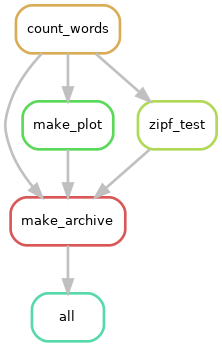
\includegraphics[width=0.4\textwidth]{workflows/complete_workflow.png}
\end{frame}




%%%%%%%%%%%%%%%%%%%%%%%%%%%%%%%%%%%%%%%%%%%%%%%%%%%%%%%%%%%%%%%%%%%%%%%%%%%%%%%%
%%%%%%%%%%%%%%%%%%%%%%%%%%%%%%%%%%%%%%%%%%%%%%%%%%%%%%%%%%%%%%%%%%%%%%%%%%%%%%%%
\section{Going HPC}

%%%%%%%%%%%%%%%%%%%%%%%%%%%%%%%%%%%%%%%%%%%%%%%%%%%%%%%%%%%%%%%%%%%%%%%%%%%%%%%%
\begin{frame}
  \frametitle{What is this about?}
   \question[Questions]{\begin{itemize}
                         \item How does ordinary job submission work on a cluster?
                         \item How does it work using Snakemake? (Which parameterization is necessary?)
                        \end{itemize}
                       }
   \docs[Objectives]{\begin{enumerate} 
                      \item Learn to use parameters relevant for the batch system SLURM
                     \end{enumerate}}
\end{frame}

%%%%%%%%%%%%%%%%%%%%%%%%%%%%%%%%%%%%%%%%%%%%%%%%%%%%%%%%%%%%%%%%%%%%%%%%%%%%%%%%
\section{How does Clustercomputing work?}

%%%%%%%%%%%%%%%%%%%%%%%%%%%%%%%%%%%%%%%%%%%%%%%%%%%%%%%%%%%%%%%%%%%%%%%%%%%%%%%%
\subsection*{The \slurm Scheduler}

%%%%%%%%%%%%%%%%%%%%%%%%%%%%%%%%%%%%%%%%%%%%%%%%%%%%%%%%%%%%%%%%%%%%%%%%%%%%%%%% 
\begin{frame}
  \frametitle{What is a scheduler?}
  On HPC systems you do not \emph{just start}, you need a \emph{``scheduler''}.
  So, what's that?\newline
  A scheduler (or ``batch system'') on a HPC system should\ldots
  \begin{itemize}
  \item provide an interface to help defining workflows and/or job dependencies
  \item enable automatic submission of executions
  \item provide interfaces to monitor the executions
  \item prioritise the execution order of unrelated jobs
  \end{itemize}
  \begin{columns}
    \begin{column}{0.8\linewidth}
      Since late spring 2017 we are using \slurm.
    \end{column}
    \begin{column}{0.2\linewidth}
      \begin{figure}
        \centering
        
\includegraphics[height=1.5cm,width=1.5cm]{slurm_logo.png}
      \end{figure}
    \end{column}
  \end{columns}
  \vfill
\end{frame}

%%%%%%%%%%%%%%%%%%%%%%%%%%%%%%%%%%%%%%%%%%%%%%%%%%%%%%%%%%%%%%%%%%%%%%%%%%%%%%%% 
\begin{frame}
  \frametitle{Promises, promises and even more promises}
  How does a scheduler work?
  \pause
  \begin{block}{You tell it\ldots}
    \begin{itemize}
    \item how much memory (RAM, scratch space) your job will need.\pause
    \item how much time you will spend on it.\pause
    \item how many CPUs you will need (and in which combination).\pause
    \item whether you need something special (e.g. a GPU).
    \end{itemize}
  \end{block}
  \pause \vspace{-0.2cm}
  \begin{exampleblock}{The scheduler will act:}
    \begin{itemize}
    \item It will queue up your job (and decide when it will start relative to others).\pause
    \item It will decide where your job will run physically (which hosts).\pause
    \item Eventually it will start your job (if everything was correct).
    \end{itemize}
  \end{exampleblock}
  \vfill
\end{frame}

\setcounter{preframe_handson}{\value{handson}}

%%%%%%%%%%%%%%%%%%%%%%%%%%%%%%%%%%%%%%%%%%%%%%%%%%%%%%%%%%%%%%%%%%%%%%%%%%%%%%%% 
\begin{frame}[fragile]
  \setcounter{handson}{\value{preframe_handson}}
  \frametitle{\HandsOn{Your first job script}}
  \hint{From now on, we will be scripting examples (cloze-based). For this you will
        need an editor. If you do not know any other editor, use \texttt{gedit}:}
  \begin{lstlisting}[language=Bash, style=Shell, basicstyle=\scriptsize]
$ # cd into appropriate directory
$ # Start gedit with the command 
$ gedit &
  \end{lstlisting}
  \hint{The \texttt{\&} will put the editor into the background.} 
\end{frame}

%%%%%%%%%%%%%%%%%%%%%%%%%%%%%%%%%%%%%%%%%%%%%%%%%%%%%%%%%%%%%%%%%%%%%%%%%%%%%%%% 
\begin{frame}[fragile]
  \setcounter{handson}{\value{preframe_handson}}
  \frametitle{\HandsOn{Your first job script}}
  \vspace{-2em}
  \begin{minipage}[t][0.32\textheight][t]{1.0\linewidth}
  \begin{lstlisting}[language=Bash, style=Shell, basicstyle=\scriptsize]
#!/bin/bash

#SBATCH -A m2_jgu-ngstraining
#SBATCH -p smp

srun echo "Hello World from job $SLURM_JOB_ID on node $(hostname)"
\end{lstlisting}
\end{minipage}\newline
\begin{minipage}[t][0.3\textheight][t]{1.0\linewidth}
  \begin{onlyenv}<1>
    \task{
    Save the script as \texttt{hello\_world.sh} and submit it with the following statement:}
    \begin{lstlisting}[language=Bash, style=Shell, basicstyle=\footnotesize]
$ sbatch hello_world.sh
\end{lstlisting}
\end{onlyenv}
\begin{onlyenv}<2>
\begin{block}{Important Items and Aspects}
  \begin{itemize}
  \item Interpreter directive
  \item Account necessary
  \item Reservation only during course
  \item Job step with \texttt{srun}
  \item Question: Where is the output?
  \end{itemize}
\end{block}
\end{onlyenv}
\end{minipage}
\vfill
\end{frame}

%%%%%%%%%%%%%%%%%%%%%%%%%%%%%%%%%%%%%%%%%%%%%%%%%%%%%%%%%%%%%%%%%%%%%%%%%%%%%%%% 
\begin{frame}
  \frametitle{End of HPC Intro}
  We could co on with \emph{many} details with regards to the scheduler, the file system, etc..
  \begin{block}{HPC Courses}
   The HPC teams offers courses to:
   \begin{itemize}
    \item HPC Intro
    \item Bash Intro
    \item Research Data Management
    \item lots of more (hopefully)
   \end{itemize}
  \end{block}
  \pause
  \hint[What's next]{We are going to parameterize our workflow\textbf{s} for clusters and for our applications in \texttt{Snakemake}!}
\end{frame}


%%%%%%%%%%%%%%%%%%%%%%%%%%%%%%%%%%%%%%%%%%%%%%%%%%%%%%%%%%%%%%%%%%%%%%%%%%%%%%%%
\section{Parametizing your Workflow}

%%%%%%%%%%%%%%%%%%%%%%%%%%%%%%%%%%%%%%%%%%%%%%%%%%%%%%%%%%%%%%%%%%%%%%%%%%%%%%%%
\subsection{Command Line vs. Configuration File}

%%%%%%%%%%%%%%%%%%%%%%%%%%%%%%%%%%%%%%%%%%%%%%%%%%%%%%%%%%%%%%%%%%%%%%%%%%%%%%%%
\begin{frame}
  \docs{\texttt{Snakemake} has an extensive command line interface (CLI). \emph{Everything} can be configured on the command line. In addition (almost) everything can be specified in a configuration file.}
  \pause
  \begin{exampleblock}{Which parameter goes where? Some rules of thumb}
    \begin{columns}[t]
      \begin{column}{0.5\textwidth}
        The CLI:
        \begin{itemize}
         \item frequently changing parameters
         \item short parameters
         \item default parameters
        \end{itemize}
      \end{column}
      \begin{column}{0.5\textwidth}
        The Config File:
        \begin{itemize}
         \item non-volantile parameters specific to your analysis (those which merit mentioning in paper should always go into a file)
         \item long parameters
         \item otherwise workflow specific parameters
        \end{itemize}
      \end{column}
    \end{columns}
  \end{exampleblock}
\end{frame}


%%%%%%%%%%%%%%%%%%%%%%%%%%%%%%%%%%%%%%%%%%%%%%%%%%%%%%%%%%%%%%%%%%%%%%%%%%%%%%%%
\subsection{The Command Line}

%%%%%%%%%%%%%%%%%%%%%%%%%%%%%%%%%%%%%%%%%%%%%%%%%%%%%%%%%%%%%%%%%%%%%%%%%%%%%%%%
\begin{frame}[fragile]
  \frametitle{Executor Selection}
  \texttt{Snakemake} lets you select various executors. Not happy with \mogon? Take another cluster or \lhref{https://snakemake.readthedocs.io/en/stable/executor_tutorial/tutorial.html}{Google Lifescience, Tibanna, Kubernetes, \ldots} \newline
  We may happily select the most prominent HPC batch system, the one running on \mogon, too:
  \begin{lstlisting}[language=Bash, style=Shell]
$ snakemake --slurm
  \end{lstlisting}
  Now, \emph{every} rule will submit its jobs as HPC compute jobs.
  \hint{We will learn how to avoid this, soon-ish.}
\end{frame}

%%%%%%%%%%%%%%%%%%%%%%%%%%%%%%%%%%%%%%%%%%%%%%%%%%%%%%%%%%%%%%%%%%%%%%%%%%%%%%%%
\begin{frame}[fragile]
  \frametitle{Default Resources for \texttt{SLURM}}
  Without specifying our SLURM-account and a (default) partition, submitting batch jobs will fail. \texttt{Snakemake} allows to define so-called default resources (using \altverb{--default-resources}). With them our minimal command line becomes:
  \begin{lstlisting}[language=Bash, style=Shell, breaklines=true]
$ snakemake --slurm \
> --default-resources slurm_account=m2_zdvhpc \
>                     slurm_partition=smp
  \end{lstlisting}
  \hint{Please notice the missing quotation marks! All arguments belong to one parameter.}
\end{frame}

%%%%%%%%%%%%%%%%%%%%%%%%%%%%%%%%%%%%%%%%%%%%%%%%%%%%%%%%%%%%%%%%%%%%%%%%%%%%%%%%
\begin{frame}[fragile]
  \frametitle{The Beauty of Clusters}
  A HPC cluster:
  \begin{itemize}
   \item offers great resources
   \item may hold jobs pending until resources are available!
  \end{itemize}
  \pause
  \texttt{Snakemake} of a semaphore throtteling resource usage, called \altverb{--jobs/-j}. We can now write \altverb{-j unlimited} in place for \altverb{--cores 1}. Let us try
  \begin{lstlisting}[language=Bash, style=Shell, breaklines=true]
$ snakemake --slurm \
> --default-resources slurm_account=m2_zdvhpc \
>                     slurm_partition=smp
> -j unlimited
  \end{lstlisting}
  together.
  \hint{You might want to invoke the \texttt{clean}-rule, first.}
\end{frame}

%%%%%%%%%%%%%%%%%%%%%%%%%%%%%%%%%%%%%%%%%%%%%%%%%%%%%%%%%%%%%%%%%%%%%%%%%%%%%%%%
\begin{frame}[fragile]
  \frametitle{\texttt{SLURM} supporting Features of \texttt{Snakemake}}
  \texttt{Snakemake} will
  \begin{itemize}[<+->]
   \item hold track of your job status (frequency of checks can be adjusted)
   \item cancle your jobs, when itself is stopped
   \item track resource consumption (generated with \altverb{--report [FILE]})
   \item with \altverb{-j unlimited} we allow for an unlimited jumber of spawned jobs!
  \end{itemize}
  \pause
  \warning{Unlimited number of jobs may yield in I/O contention and too many calls to check the job status. Use with care for both issues there is a remedy!}
\end{frame}

%%%%%%%%%%%%%%%%%%%%%%%%%%%%%%%%%%%%%%%%%%%%%%%%%%%%%%%%%%%%%%%%%%%%%%%%%%%%%%%%
\subsection{The Configuration File}

%%%%%%%%%%%%%%%%%%%%%%%%%%%%%%%%%%%%%%%%%%%%%%%%%%%%%%%%%%%%%%%%%%%%%%%%%%%%%%%%
\begin{frame}[fragile]
  \frametitle{The \texttt{Snakemake} \texttt{resources} Section}
  \texttt{Snakemake} rules provide an additional \altverb{resource} section:
  \begin{lstlisting}[language=Python,style=Python]
rule <name>:
   ...
   resources:
      partition='parallel',
      mem_mb=1800,
      cpus_per_task=4
  \end{lstlisting}
  \hint{Note the \textbf{,}!}
  \pause
  \docs{You \emph{may} define \emph{any} resource keyword within any rule.}
\end{frame}

%%%%%%%%%%%%%%%%%%%%%%%%%%%%%%%%%%%%%%%%%%%%%%%%%%%%%%%%%%%%%%%%%%%%%%%%%%%%%%%%
\begin{frame}
  \frametitle{The Configuration File}
  If observed closely you have seen this file:\newline
            {\tiny \DTsetlength{0.2em}{1em}{0.2em}{0.4pt}{.6pt}
\texttt{\$ tree}
\dirtree{%
.1 /.
.2 config.
.3 samples.yaml .
.2 {other stuff}.
}}
 \pause
 \docs{You can store a yaml file with \emph{your} workflow configuration -- which may be combined with the desinger's configuration.}
\end{frame}

%%%%%%%%%%%%%%%%%%%%%%%%%%%%%%%%%%%%%%%%%%%%%%%%%%%%%%%%%%%%%%%%%%%%%%%%%%%%%%%%
\begin{frame}[fragile]
  \frametitle{Using the Configuration File}
  To point to the configuration file, you can add a flag, e.\,g.:
  \begin{lstlisting}[language=Bash, style=Shell]
$ snakemake ... --configfile ./config/samples.yaml  
  \end{lstlisting}
  Yet, you have seen its contents?
  \begin{lstlisting}[language=Bash, style=Shell]
$ cat ./config/samples.yaml
path: '~/workflows/books'
limit: 10
  \end{lstlisting}
  \question{How do pick up resource parameters in out \texttt{Snakefile}?!}
\end{frame} 

\begin{frame}[fragile]
  \frametitle{\Interlude{Introducing Python's \texttt{os} Library}}
  Python has a library to provide functions to deal with operating systems, including file systems. Check out:
  \begin{lstlisting}[language=Python,style=Python]
>>> import os
>>> path = "~/workflows/books"
>>> os.realpath(path)

  \end{lstlisting}

\end{frame}


%%%%%%%%%%%%%%%%%%%%%%%%%%%%%%%%%%%%%%%%%%%%%%%%%%%%%%%%%%%%%%%%%%%%%%%%%%%%%%%%
\begin{frame}[fragile]
  \frametitle{Using the Configuration File - II}
  Within our \texttt{Snakefile} we can access our configuration as any Python dictionary:
  \begin{lstlisting}[language=Python,style=Python]
input_path = config["path"]
  \end{lstlisting}
  \hint{This, however, is useless: if our \texttt{path} is a relative path, every derived path is relative to our current working directory!}
  \pause
  Lukily, \texttt{Snakefile}s are Python-Code:
  \begin{lstlisting}[language=Python,style=Python]
import os

input_path  = os.path.realpath(config['path'])
output_path = os.path.join('results', 
                           os.path.dirname(input_path))

DATS = glob_wildcards(os.path.join(input_path, 
                      "{book}.txt")).book
  \end{lstlisting}
  
\end{frame}

%%%%%%%%%%%%%%%%%%%%%%%%%%%%%%%%%%%%%%%%%%%%%%%%%%%%%%%%%%%%%%%%%%%%%%%%%%%%%%%%
\begin{frame}[fragile]
  \frametitle{Our Workflow}
  \task{Add the following resource to our workflow.}
  \begin{lstlisting}[language=Python,style=Python]
   resources:
      mem_mb=1800
  \end{lstlisting}
  \question{Why? Why not more?}
  \pause
  Because,
  \begin{itemize}
   \item \texttt{ntasks} and \texttt{cpus\_per\_task} default to 1, which is the case here.
   \item account and partition are the same everywhere and we can use this upon submit time (see next slide)
   \item \texttt{mem\_mb} is the same everywhere, too. But: it is usually a resource to be adapter per rule. So, we try this here, too.
  \end{itemize}
\end{frame}

%%%%%%%%%%%%%%%%%%%%%%%%%%%%%%%%%%%%%%%%%%%%%%%%%%%%%%%%%%%%%%%%%%%%%%%%%%%%%%%%
\begin{frame}[fragile]
  \frametitle{Starting our Workflow - One last Time}
  \begin{lstlisting}[language=Bash,style=Shell]
$ snakemake -j unlimited --use-envmodules --slurm \
  --default-ressources account=hpckurs partition=smp
  \end{lstlisting}
  \question{Which warning(s) do turn up? What is the remedy?}
\end{frame}

%%%%%%%%%%%%%%%%%%%%%%%%%%%%%%%%%%%%%%%%%%%%%%%%%%%%%%%%%%%%%%%%%%%%%%%%%%%%%%%%
\begin{frame}[fragile]
  \frametitle{Configuration Files}
  Workflows, once established, should not be altered. All settings go into configuration files. To indicate a configuration file, run with:
  \begin{lstlisting}[language=Bash,style=Shell]
$ snakemake --configfile=<path>
  \end{lstlisting}\pause
  The configuration file itsels is in YAML format and might look like:
  \begin{lstlisting}[language=Python,style=Python]
INPUT_DIR: "/lustre/project/..."
OUTPUT_DIR: "/lustre/project/..."
# environment modules:
VINALC: "bio/VinaLC/1.3.0-gompi-2021b"
  \end{lstlisting}\pause
    Within the Snakefile we can retrieve this information, as it is represented as Python \texttt{dicts}:
  \begin{columns}
     \begin{column}{0.5\textwidth}
       \begin{lstlisting}[language=Bash,style=Shell,basicstyle=\small]
INPUT_DIR=config["INPUT_DIR"]
OUTPU_DIR=config["OUTPUT_DIR"]
       \end{lstlisting}
     \end{column}
     \begin{column}{0.5\textwidth}
      \begin{lstlisting}[language=Bash,style=Shell,basicstyle=\small] 
rule NAME:HPC_Parameterization.tex
    ...
    envmodules:
       config["VINALC"]    
      \end{lstlisting}

     \end{column}
  \end{columns}

\end{frame}





%%%%%%%%%%%%%%%%%%%%%%%%%%%%%%%%%%%%%%%%%%%%%%%%%%%%%%%%%%%%%%%%%%%%%%%%%%%%%%%%

\end{document}

